\documentclass[10pt,conference]{IEEEtran}
\usepackage{makecell, multirow, url}
\usepackage{pifont}
\usepackage[table]{xcolor}
\usepackage{graphicx}
\usepackage{amsmath}
\usepackage{microtype}
\usepackage{array}
\usepackage{enumitem}
\usepackage{booktabs}
\usepackage{colortbl}
\usepackage{tikz}
\usetikzlibrary{patterns,decorations.pathreplacing,positioning,matrix}
\usepackage{pgfplots}
\usepgfplotslibrary{groupplots}
\pgfplotsset{compat=1.18}

\setlength{\aboverulesep}{0.5pt}
\setlength{\belowrulesep}{0.5pt}
\setlength{\cmidrulekern}{2pt}
\setlength{\emergencystretch}{1em}
\hyphenpenalty=1000
\exhyphenpenalty=1000
\hyphenation{light-weight}

\title{Budget-Aware Draft Admission and Capture Pacing: \\ Coordinated Capture-Timeout Prevention in a Commercial Samsung Camera Framework}
% \affil{Anonymous Affiliation}

\author{
  \IEEEauthorblockN{Minhyun Park}
  \IEEEauthorblockA{\textit{Samsung Electronics}\\
  \textit{Sungkyunkwan University}\\
  Suwon, Republic of Korea\\
  mhyun2.park@samsung.com}
  
  \and 
  
  \IEEEauthorblockN{Sooyoung Cha}
  \thanks{Corresponding author}
  \IEEEauthorblockA{\textit{Sungkyunkwan University}\\
  Suwon, Republic of Korea\\
  sooyoung.cha@skku.edu}
}

\begin{document}
\pagestyle{plain}

\maketitle

% Shared macros used by the current camera-framework manuscript.

% Short condition label used in the evaluation tables.
\newcommand{\memory}{{\it mem}}

% Fit a tabular to an exact target width by iteratively solving for
% \tabcolsep.  #4 is twice the number of columns.
\newcommand{\fittabcolsepstep}[4]{%
  \sbox{#1}{#2}\addtolength{\tabcolsep}{\dimexpr(#3-\wd#1)/#4\relax}}
\newcommand{\fittabcolsep}[4]{%
  \setlength{\tabcolsep}{0pt}%
  \fittabcolsepstep{#1}{#2}{#3}{#4}\fittabcolsepstep{#1}{#2}{#3}{#4}%
  \fittabcolsepstep{#1}{#2}{#3}{#4}\fittabcolsepstep{#1}{#2}{#3}{#4}%
  \fittabcolsepstep{#1}{#2}{#3}{#4}\fittabcolsepstep{#1}{#2}{#3}{#4}%
  \fittabcolsepstep{#1}{#2}{#3}{#4}\fittabcolsepstep{#1}{#2}{#3}{#4}}

\begin{abstract}
% We present the Budget-Aware Draft Controller, which enables lightweight multi-frame composition in the draft pipeline of Samsung Galaxy cameras under parallel capture and a hard per-capture deadline, the Capture Timeout.
% For selected shot modes, post-processing is deferred until the application enters the background, so the initial draft image remains the user-visible result throughout the foreground session, making its visual quality more important.
% However, lightweight multi-frame composition can violate the Capture Timeout, and under parallel capture, where draft sequences execute one at a time, its added processing also consumes the timeout budget of every capture queued behind it.
% The production thermal guard skips optional stages at a fixed overheat level and therefore cannot separate safe captures from unsafe ones.
% Our controller coordinates two runtime decisions: remaining-sequence admission decides whether to execute each optional stage, and capture-availability pacing decides whether to delay the next capture.
% One major challenge is that both decisions depend on draft work not yet executed; to address this, the controller estimates stage durations online from completed draft sequences.
% Across 28 combinations of two devices, two capture conditions, and seven starting overheat levels, no controller run of 30 captures reached Capture Timeout, whereas running every optional stage without the guard did so in 26 combinations.
% In combinations starting at overheat level 4 or higher, where the guard would skip optional stages, lightweight multi-frame composition still executed on an average of 5.2--22.2 of 30 captures per run.
% The controller is undergoing release validation for a forthcoming Galaxy flagship smartphone line.
\end{abstract}
\section{Introduction}

\label{sec:introduction}

% Samsung Galaxy camera capture pipelines publish an initial image before post-processing produces the final image.
% We refer to the pipeline that produces this initial image as the draft sequence.
% For selected modes, post-processing begins only after the application enters the background, prolonging the period for which the initial image remains visible.
% We therefore added lightweight multi-frame composition to the draft sequence to reduce the visible gap to the final image.

% Each capture must produce its initial image within a fixed deadline.
% A violation of this deadline is referred to as a Capture Timeout.
% Parallel capture turns this per-capture deadline into a cross-capture control problem.
% The application may accept a new shutter request before the preceding initial image is produced, while draft sequences execute in capture order on a single worker.
% Work admitted for one capture therefore increases the waiting time of subsequent captures and reduces their remaining deadline budgets.

% The production system limits this risk by disabling optional processing in the draft sequence at a fixed overheat level.
% Thermal level, however, does not reflect queueing time, remaining work, or remaining deadline budget.
% The cutoff can suppress feasible work at or above the threshold while leaving timeout risk below it unaddressed.

% Workload adaptation and request-release control are established responses to latency and queueing pressure~\cite{approxdet-sensys,timecard-sosp,seda-sosp,breakwater-osdi}.
% In our pipeline, neither is sufficient alone: workload control cannot prevent the next capture from joining a busy worker, while release control cannot reduce work already admitted for the current capture.
% We therefore present the Budget-Aware Draft Controller, which coordinates \emph{Remaining-Sequence Admission} with \emph{Capture-Availability Pacing}.
% Admission allows an optional stage only when an upper estimate of the work remaining before initial-image publication, including mandatory encoding and saving, fits within the capture's remaining deadline budget.
% Pacing delays the next capture opportunity when projected worker occupancy would leave too little deadline budget for the next capture.
% Both decisions use observed processing durations rather than per-model timing tables or thermal-state signals.

% The two controls incur different costs.
% Pacing directly lengthens the shot-to-shot interval, whereas skipping an optional stage affects only the initial image until the final image replaces it.
% The controller therefore prioritizes responsiveness while preserving optional processing when the remaining deadline budget permits.

% Across 28 combinations of two devices, two capture conditions, and seven starting overheat levels, every run with the full controller completed the 30-capture horizon without an observed Capture Timeout.
% The unguarded baseline reached Capture Timeout in 26 of the 28 cells.
% The controller continued to execute lightweight multi-frame composition even at or above the production thermal cutoff.
% Only the full controller completed every requested capture on time in all evaluated ablation cells.

% \smallskip\noindent\textbf{Contributions.}
% We summarize our contributions below:
% \begin{itemize}[leftmargin=1.2em]
%   \item We characterize how serialized Draft execution under parallel capture creates a cross-capture deadline problem for lightweight multi-frame composition, and show why a static thermal cutoff does not reflect per-capture deadline safety.
%   \item We present the Budget-Aware Draft Controller, which coordinates remaining-sequence admission with next-capture pacing using runtime duration observations. To our knowledge, this is the first production camera controller to combine these controls under a hard per-capture deadline.
%   \item We evaluate the controller on two commercial devices across 28 device--condition--thermal combinations, examining end-to-end effectiveness, control-loop contribution, admission quality, and pacing-delay sizing.
% \end{itemize}
% Chapter 2: Background and problem characterization.
% Sources: docs/Motivation.txt and docs/research-context.md.

\providecommand{\deadline}{\ensuremath{D}}
\providecommand{\queuewait}{\ensuremath{q}}
\providecommand{\dur}{\ensuremath{T}}
\providecommand{\admitted}{\ensuremath{A}}

\section{Background and Problem Characterization}\label{sec:background}

\subsection{Draft Delivery and Deferred Processing}\label{sec:draft-background}

One shutter event produces multiple buffers that the full post-processing
path collects, fuses, encodes, and saves. The companion Draft path selects its
input earlier, publishes a media-database entry, and retains a recovery image;
the final result later replaces that entry. These paths were designed
together, but the work inside the Draft changed. An effect-free Draft first
gained single-frame Filter and Watermark to resemble the final image. The next
attempted extension was lightweight multi-frame Draft Bokeh for portrait
capture.

Figure~\ref{fig:draft-pipeline} explains why this richer Draft became
necessary. Increasingly expensive processing competes with foreground preview
and capture preparation, so selected modes wait for the application to enter
the background before final composition. Portrait originally composed in the
foreground despite its high cost and large before--after difference. Draft
Bokeh was intended to provide an approximate portrait during this interval and
thereby enable the heavy final portrait composition to be deferred. Repeated
Capture Timeout blocked this transition in two flagship generations.

\begin{figure}[t]
  \centering
  % Companion draft and final paths in the camera post-processing pipeline.
% Included from _2_preliminary.tex.
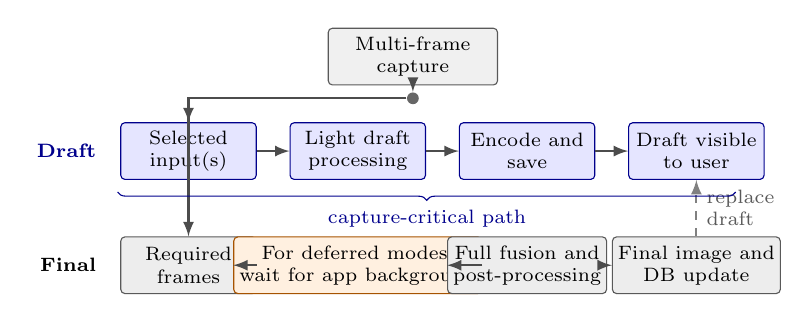
\begin{tikzpicture}[
  font=\scriptsize,
  >=latex,
  box/.style={draw=black!65, rounded corners=1.5pt, align=center,
    minimum width=1.72cm, minimum height=0.72cm, inner sep=2pt},
  draft/.style={box, draw=blue!55!black, fill=blue!10},
  final/.style={box, draw=black!65, fill=gray!14},
  gate/.style={box, draw=orange!65!black, fill=orange!12},
  flow/.style={->, thick, black!70},
  split/.style={circle, fill=black!60, inner sep=1.5pt}
]

  \node[box, fill=black!6, minimum width=2.15cm] (capture) at (3.85,3.55)
    {Multi-frame\\capture};
  \node[split] (fork) at (3.85,3.02) {};
  \draw[flow] (capture) -- (fork);

  % Draft lane.
  \node[anchor=east, font=\scriptsize\bfseries, text=blue!55!black]
    at (-0.05,2.35) {Draft};
  \node[draft] (dinput) at (1.00,2.35) {Selected\\input(s)};
  \node[draft] (deffect) at (3.15,2.35) {Light draft\\processing};
  \node[draft] (dsave) at (5.30,2.35) {Encode and\\save};
  \node[draft] (dvisible) at (7.45,2.35) {Draft visible\\to user};

  \draw[flow] (fork) -| (dinput.north);
  \draw[flow] (dinput) -- (deffect);
  \draw[flow] (deffect) -- (dsave);
  \draw[flow] (dsave) -- (dvisible);

  % Final lane.
  \node[anchor=east, font=\scriptsize\bfseries] at (-0.05,0.90) {Final};
  \node[final] (finput) at (1.00,0.90) {Required\\frames};
  \node[gate] (fgate) at (3.15,0.90) {For deferred modes:\\wait for app background};
  \node[final] (fprocess) at (5.30,0.90) {Full fusion and\\post-processing};
  \node[final] (fupdate) at (7.45,0.90) {Final image and\\DB update};

  \draw[flow] (fork) -| (finput.north);
  \draw[flow] (finput) -- (fgate);
  \draw[flow] (fgate) -- (fprocess);
  \draw[flow] (fprocess) -- (fupdate);

  % The final result replaces the published draft entry.
  \draw[flow, dashed, black!50] (fupdate.north) -- (dvisible.south)
    node[midway, right, align=left, text=black!65] {replace\\draft};

  \draw[decorate, decoration={brace, mirror, amplitude=3pt}, blue!55!black]
    (0.10,1.83) -- (7.95,1.83);
  \node[anchor=north, text=blue!55!black] at (4.03,1.72)
    {capture-critical path};

\end{tikzpicture}

  \caption{Intended portrait transition: Draft Bokeh places a lightweight
  approximation on the deadline-critical Draft path, permitting heavy final
  composition to wait for the application background. $D$ marks the Draft
  delivery deadline.}
  \label{fig:draft-pipeline}
\end{figure}

\subsection{Parallel Capture Turns Latency into Backlog}\label{sec:timeout}

\emph{Capture Timeout} occurs when capture processing, including Draft
delivery, misses the framework's fixed 7-second deadline \deadline. Parallel
capture changed how that deadline is consumed. The HAL may issue
\texttt{captureAvailable} before the preceding Draft completes, allowing the
application to start another capture. Draft Sequences nevertheless share a
single worker.

Figure~\ref{fig:overlap} shows the result. The Draft for capture $i{+}1$ waits
behind capture $i$'s Draft, and the Draft for capture $i{+}2$ waits behind
both. Because each deadline starts at its capture rather than at its Draft
execution, queueing removes budget before any work for that image begins. One
tail-latency spike can therefore cause a later capture to time out even when
every capture executes the same stages.

\begin{figure}[t]
  \centering
  \resizebox{\columnwidth}{!}{% Timeline of two draft sequences overlapping under parallel capture.
% Included from _2_preliminary.tex (Figure~\ref{fig:overlap}).
% Requires: tikz with libraries `patterns' and `decorations.pathreplacing';
% pifont for the check mark.
%
% Design: both captures run the identical stage sequence
% [Bokeh][other][Filter][other][Encode]. Capture i meets its deadline with
% slack; capture i+1 inherits queueing delay from the single draft thread,
% so the same workload overruns its deadline during the mandatory encode.
% Only Bokeh, Filter, and Encode are named; the two remaining draft stages
% are anonymized as short gray "other" stages marked `A' and `B' (their
% durations are small).
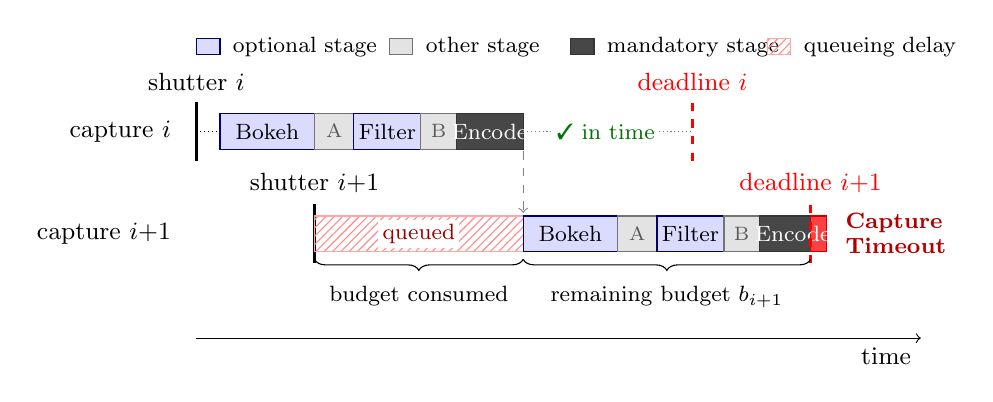
\begin{tikzpicture}[font=\small,
  optstage/.style={draw=blue!45!black, fill=blue!14},
  othstage/.style={draw=black!55, fill=gray!22},
  encstage/.style={draw=black!80, fill=black!72},
  queued/.style={pattern=north east lines, pattern color=red!45, draw=red!35},
  ddl/.style={red, dashed, thick}]

  % ---------- legend (top) ----------
  \draw[optstage] (0, 3.2) rectangle (0.3, 3.4);
  \node[anchor=west] at (0.34, 3.3) {\footnotesize optional stage};
  \draw[othstage] (2.45, 3.2) rectangle (2.75, 3.4);
  \node[anchor=west] at (2.79, 3.3) {\footnotesize other stage};
  \draw[encstage] (4.75, 3.2) rectangle (5.05, 3.4);
  \node[anchor=west] at (5.09, 3.3) {\footnotesize mandatory stage};
  \draw[queued] (7.25, 3.2) rectangle (7.55, 3.4);
  \node[anchor=west] at (7.59, 3.3) {\footnotesize queueing delay};

  % ---------- capture i (top row) ----------
  \node[anchor=east] at (-0.2, 2.225) {capture $i$};
  % shutter marker
  \draw[very thick] (0, 1.85) -- (0, 2.6);
  \node[anchor=south] at (0, 2.62) {shutter $i$};
  % lead-in until the draft frame is available
  \draw[densely dotted] (0, 2.225) -- (0.3, 2.225);
  % draft sequence i
  \draw[optstage] (0.3, 2.0) rectangle (1.5, 2.45);
  \node at (0.9, 2.225) {\footnotesize Bokeh};
  \draw[othstage] (1.5, 2.0) rectangle (2.0, 2.45);
  \node at (1.75, 2.225) {\scriptsize\textcolor{black!65}{A}};
  \draw[optstage] (2.0, 2.0) rectangle (2.85, 2.45);
  \node at (2.425, 2.225) {\footnotesize Filter};
  \draw[othstage] (2.85, 2.0) rectangle (3.3, 2.45);
  \node at (3.075, 2.225) {\scriptsize\textcolor{black!65}{B}};
  \draw[encstage] (3.3, 2.0) rectangle (4.15, 2.45);
  \node at (3.725, 2.225) {\footnotesize\textcolor{white}{Encode}};
  % slack before deadline i
  \draw[densely dotted, gray] (4.15, 2.225) -- (6.3, 2.225);
  \node[fill=white, inner sep=1.5pt] at (5.2, 2.225)
    {\footnotesize\textcolor{green!45!black}{\ding{51} in time}};
  % deadline of capture i
  \draw[ddl] (6.3, 1.85) -- (6.3, 2.6);
  \node[red, anchor=south] at (6.3, 2.62) {deadline $i$};

  % ---------- capture i+1 (bottom row) ----------
  \node[anchor=east] at (-0.2, 0.925) {capture $i{+}1$};
  % shutter marker (accepted while draft sequence i is still running)
  \draw[very thick] (1.5, 0.55) -- (1.5, 1.3);
  \node[anchor=south] at (1.5, 1.32) {shutter $i{+}1$};
  % queueing behind draft sequence i
  \draw[queued] (1.5, 0.7) rectangle (4.15, 1.15);
  \node[fill=white, inner sep=1.5pt] at (2.825, 0.925)
    {\footnotesize\textcolor{red!60!black}{queued}};
  % draft sequence i+1 (identical stage durations)
  \draw[optstage] (4.15, 0.7) rectangle (5.35, 1.15);
  \node at (4.75, 0.925) {\footnotesize Bokeh};
  \draw[othstage] (5.35, 0.7) rectangle (5.85, 1.15);
  \node at (5.6, 0.925) {\scriptsize\textcolor{black!65}{A}};
  \draw[optstage] (5.85, 0.7) rectangle (6.7, 1.15);
  \node at (6.275, 0.925) {\footnotesize Filter};
  \draw[othstage] (6.7, 0.7) rectangle (7.15, 1.15);
  \node at (6.925, 0.925) {\scriptsize\textcolor{black!65}{B}};
  \draw[encstage] (7.15, 0.7) rectangle (8.0, 1.15);
  % overrun beyond deadline i+1 (drawn before the label so the text stays visible)
  \draw[draw=red!80!black, fill=red!75] (7.8, 0.7) rectangle (8.0, 1.15);
  \node at (7.575, 0.925) {\footnotesize\textcolor{white}{Encode}};
  % deadline of capture i+1 (crosses the mandatory encode)
  \draw[ddl] (7.8, 0.55) -- (7.8, 1.3);
  \node[red, anchor=south] at (7.8, 1.32) {deadline $i{+}1$};
  % timeout callout
  \node[red!70!black, anchor=west, align=left] at (8.12, 0.925)
    {\footnotesize\bfseries Capture\\[-2pt]\footnotesize\bfseries Timeout};

  % ---------- single-thread handoff ----------
  % Drawn after both rows so the arrowhead is not overpainted by the box
  % borders; the label sits to the right of the arrow.
  \draw[dashed, gray, ->] (4.15, 1.97) -- (4.15, 1.19);
  \node[anchor=west] at (4.27, 1.5)
    {\footnotesize\textcolor{gray}{}};

  % ---------- budget braces ----------
  \draw[decorate, decoration={brace, mirror, amplitude=4pt}]
    (1.5, 0.6) -- (4.15, 0.6);
  \node[anchor=north] at (2.825, 0.38) {\footnotesize budget consumed};
  \draw[decorate, decoration={brace, mirror, amplitude=4pt}]
    (4.15, 0.6) -- (7.8, 0.6);
  \node[anchor=north] at (5.975, 0.38) {\footnotesize remaining budget $b_{i+1}$};

  % ---------- time axis ----------
  \draw[->] (0, -0.4) -- (9.2, -0.4) node[anchor=north east] {time};

\end{tikzpicture}
}
  \caption{Parallel captures queue on one Draft worker. Successive captures
  start Draft execution with less remaining budget until capture $i{+}2$
  reaches its deadline during mandatory encoding.}
  \label{fig:overlap}
\end{figure}

\subsection{Why Level~4 Is Not a Safety Boundary}\label{sec:guard-limit}

The deployed policy originated as an Lv5 response to high-level Draft failures
and was tightened to Lv4 after a lower-tier Filter timeout; shared framework
code applied the same rule to flagships. It disables every optional Draft
stage at Lv4 and above, irrespective of the configured sequence or queue
state. This was a reasonable release safeguard, but
Table~\ref{tab:timeout_index} illustrates its two errors in our motivating
characterization on a flagship device. The table forces the indicated Bokeh
and Filter configurations at every level and reports the first timeout in a
30-shot portrait burst.

% Notes: docs/exhibits.md#tab_timeout_index
\providecolor{tmoS1}{RGB}{252,227,220} %
\providecolor{tmoS2}{RGB}{239,160,140} %
\providecolor{tmoS3}{RGB}{201,80,63}  %
\providecolor{tmoS4}{RGB}{143,36,32}  %

\newcolumntype{H}{>{\centering\arraybackslash}m{1.20cm}}
\newcolumntype{P}{>{\centering\arraybackslash}m{0.67cm}}

\providecommand{\tmoFirst}[2]{\cellcolor{#1}\makebox[\linewidth][r]{#2\hspace{1pt}}}
\providecommand{\tmoFirstW}[2]{\cellcolor{#1}\makebox[\linewidth][r]{\textcolor{white}{\textbf{#2}}\hspace{1pt}}}
\providecommand{\tmoNone}{\makebox[\linewidth][r]{--\hspace{1pt}}}

\begin{table}[t]
 \centering
 \caption{Earliest Timeout onset across capture conditions.}
 \label{tab:timeout_index}
 {\scriptsize\setlength{\tabcolsep}{1.3pt}%
 \begin{tabular}{@{}HPP|PP||PP|PP@{}}
 \toprule
 \multirow[c]{3}{=}[-10pt]{\makecell[c]{\textbf{Starting}\\\textbf{overheat}\\\textbf{level}}} &
 \multicolumn{4}{c||}{\raisebox{-3pt}{\textbf{Normal capture}}} &
 \multicolumn{4}{c@{}}{\raisebox{-3pt}{\textbf{Memory-pressure capture}}} \\[6pt] \cmidrule(lr){2-5}\cmidrule(l){6-9}
 &
 \multicolumn{2}{c|}{\raisebox{-3pt}{\textbf{12MP}}} &
 \multicolumn{2}{c||}{\raisebox{-3pt}{\textbf{24MP}}} &
 \multicolumn{2}{c|}{\raisebox{-3pt}{\textbf{12MP}}} &
 \multicolumn{2}{c@{}}{\raisebox{-3pt}{\textbf{24MP}}} \\[6pt] \cmidrule(lr){2-3}\cmidrule(lr){4-5}\cmidrule(lr){6-7}\cmidrule(l){8-9}
 & \raisebox{-2pt}{\textbf{M{+}S}} & \raisebox{-2pt}{\textbf{M}} &
 \raisebox{-2pt}{\textbf{M{+}S}} & \raisebox{-2pt}{\textbf{M}} &
 \raisebox{-2pt}{\textbf{M{+}S}} & \raisebox{-2pt}{\textbf{M}} &
 \raisebox{-2pt}{\textbf{M{+}S}} & \raisebox{-2pt}{\textbf{M}} \\[4pt]
 \midrule
 Lv0 &
 \tmoNone & \tmoNone & \tmoFirst{tmoS1}{29} & \tmoNone &
 \tmoNone & \tmoNone & \tmoFirst{tmoS1}{26} & \tmoNone \\
 Lv1 &
 \tmoNone & \tmoNone & \tmoFirst{tmoS1}{29} & \tmoNone &
 \tmoFirst{tmoS1}{24} & \tmoNone & \tmoFirst{tmoS2}{19} & \tmoNone \\
 Lv2 &
 \tmoFirst{tmoS1}{24} & \tmoNone & \tmoFirst{tmoS2}{18} & \tmoNone &
 \tmoFirst{tmoS2}{15} & \tmoFirst{tmoS1}{29} &
 \tmoFirst{tmoS2}{14} & \tmoFirst{tmoS1}{25} \\
 Lv3 &
 \tmoFirst{tmoS2}{13} & \tmoFirst{tmoS1}{21} &
 \tmoFirst{tmoS2}{12} & \tmoFirst{tmoS1}{20} &
 \tmoFirstW{tmoS3}{8} & \tmoFirst{tmoS2}{19} &
 \tmoFirstW{tmoS4}{5} & \tmoFirst{tmoS2}{13} \\
 \midrule
 Lv4 &
 \tmoFirstW{tmoS3}{8} & \tmoFirst{tmoS2}{16} &
 \tmoFirstW{tmoS3}{7} & \tmoFirst{tmoS2}{13} &
 \tmoFirstW{tmoS3}{6} & \tmoFirst{tmoS2}{13} &
 \tmoFirstW{tmoS4}{3} & \tmoFirstW{tmoS3}{7} \\
 Lv5 &
 \tmoFirstW{tmoS3}{8} & \tmoFirst{tmoS2}{12} &
 \tmoFirstW{tmoS3}{8} & \tmoFirst{tmoS2}{12} &
 \tmoFirstW{tmoS4}{4} & \tmoFirstW{tmoS3}{9} &
 \tmoFirstW{tmoS4}{4} & \tmoFirstW{tmoS3}{9} \\
 Lv6 &
 \tmoFirstW{tmoS3}{7} & \tmoFirst{tmoS2}{11} &
 \tmoFirstW{tmoS3}{7} & \tmoFirst{tmoS2}{11} &
 \tmoFirstW{tmoS4}{3} & \tmoFirstW{tmoS3}{6} &
 \tmoFirstW{tmoS4}{3} & \tmoFirstW{tmoS3}{6} \\
 \bottomrule
 \end{tabular}%
 }
 \par\vspace{3pt}
 {\scriptsize\begin{minipage}{0.933\columnwidth}
 \raggedright\setlength{\fboxsep}{1.8pt}%
 Earliest timeout onset:~%
 \colorbox{tmoS1}{\strut\,${\geq}\,20$\,}\colorbox{tmoS2}{\strut\,10--19\,}\colorbox{tmoS3}{\strut\,\textcolor{white}{6--9}\,}\colorbox{tmoS4}{\strut\,\textcolor{white}{${\leq}\,5$}\,}\par
 \end{minipage}}
\end{table}

First, the guard is \emph{under-protective}. Bokeh with Filter times out below
the boundary---at Lv0 for 24MP normal capture and Lv2 for 12MP normal capture.
Second, it is \emph{over-restrictive}. At Lv4, the 12MP normal trace completes
nine shots with both stages and 15 with Bokeh alone before its first timeout;
the guard would nevertheless skip optional work even for the first capture.
Overheat correlates with slowdown, but it does not encode image size, memory
pressure, workload composition, or burst backlog. No nontrivial thermal
threshold separates safe and unsafe executions in this characterization.

\subsection{Two Complementary Control Points}\label{sec:control-problem}

Let capture $i$ begin at $a_i$ and its Draft start at $s_i$, giving queueing
delay $\queuewait_i=s_i-a_i$. If $\admitted_i$ is its selected optional work,
$\dur_i(\admitted_i)$ is the duration of the resulting Draft sequence,
including all non-optional work and mandatory encoding. The deadline condition
is

\begin{equation}
  \queuewait_i + \dur_i(\admitted_i) \leq \deadline.
  \label{eq:draft-deadline}
\end{equation}

Admission controls $\dur_i(\admitted_i)$ for the current capture, but cannot
recover budget already lost to $\queuewait_i$. Pacing delays the earliest next
capture opportunity so queued work can drain, reducing future queueing at the
cost of responsiveness; it cannot prevent a tail spike after release. Meeting
all three objectives therefore calls for both controls: avoid timeout, retain
the preferred Draft path when feasible, and minimize added pacing. The next
section presents the shared tail model and the two decisions built on it.

% Chapter 3: the Budget-Aware Draft Controller.
%
% Implementation evidence: private ML repository
% (https://github.com/ParkMinhyun/ML), commit
% 99aae0af8c3fa1ceb784083446e83c40d0fb917f. Key sources:
% DraftSequenceExecutionPredictor.kt (model, admission, watchdog),
% CaptureAvailablePacer.kt (pacing), DraftSequenceExecutionProfiler.kt
% (node classification, integration), WorkloadKey.kt /
% WorkloadSequenceKey.kt (taxonomy), CaptureMetrics.kt (observability).

\section{The Budget-Aware Draft Controller}\label{sec:approach}

% \subsection{Overview and Control Objective}
\label{sec:objective}

\begin{figure*}[!t]
  \centering
  % Source PDF is 864.0 x 297.36 pt; measured ink box is x 21.1--854.9, y 12.5--285.8.
  % Trim removes the empty top/bottom bands and the 12 pt of excess left slack so the
  % remaining side margins match at 9.1 pt. Re-measure if the figure is re-exported.
  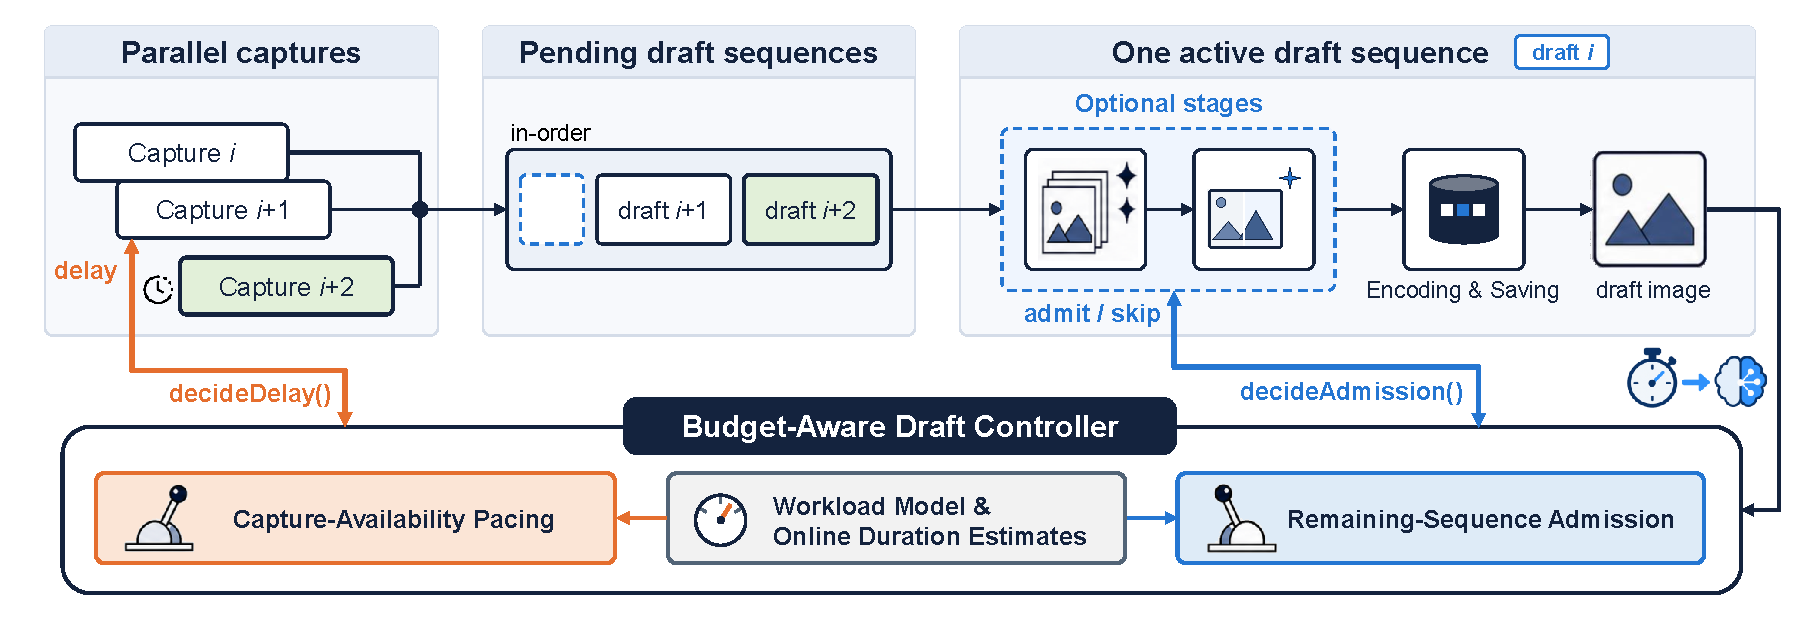
\includegraphics[trim=12 10 0 11,clip,width=\textwidth]{figures/fig_controller_interaction.pdf}
  \caption{Overview of the Budget-Aware Draft Controller.}
  \label{fig:controller-overview}
\end{figure*}
We introduce the \emph{Budget-Aware Draft Controller} to enable lightweight multi-frame composition under parallel capture while meeting each capture's deadline.

\smallskip\noindent\textbf{Controller architecture.}
The controller manages both the work occupying the single draft worker and the requests entering its queue, as shown in Figure~\ref{fig:controller-overview}.
\emph{Remaining-Sequence Admission} runs immediately before an optional stage in the active draft sequence.
It compares the estimated time for the remaining sequence with the capture's remaining timeout budget to decide whether to execute the stage.
\emph{Capture-Availability Pacing} controls delivery of \texttt{captureAvailable}, which exposes the next capture opportunity to the application.
It uses estimated worker occupancy and the remaining deadline window to decide whether to deliver the callback immediately or delay it.

Both modules learn duration estimates from the per-stage and sequence-level measurements of completed draft sequences.
Their shared runtime state connects the two decisions: when admission skips optional stages, pacing adjusts its duration reserve to reflect the stages still eligible for execution.

\smallskip\noindent\textbf{Control objective.}
Capture Timeout is a hard product constraint on enabling optional stages.
Each accepted capture starts its own deadline clock, but its Draft Sequence may wait behind earlier captures on the shared worker.
This waiting consumes the budget available for the remaining stages.
Admission can reduce the remaining processing time by skipping optional stages, but it cannot recover time already spent waiting.
Pacing can delay the next capture opportunity to let the worker progress, but it cannot change work already in progress.
At each decision, the controller compares a processing-time forecast with the live remaining timeout budget.

Within this deadline constraint, the controller prioritizes user-perceived responsiveness.
Capture delay lengthens the shot-to-shot interval and cannot be recovered, whereas the fidelity cost of a skipped stage ends when the final image replaces the draft image.
The controller therefore implements a deadline-constrained, responsiveness-dominant trade-off rather than a global cost optimization.

% \subsection{Workload Model and Online Duration Estimation}
\label{sec:model}
A Draft Sequence's duration depends on its stages and how fast they execute under current conditions.
The controller therefore learns stage durations from completed Draft Sequences and combines them according to the sequence being considered.

\smallskip\noindent\textbf{Modeled workload sequence.}
Each combination of a processing stage and its configuration is identified by a workload key \(k\).
Capture \(i\)'s Draft Sequence is represented by the ordered keys \(\mathcal{K}_i=(k_1,\ldots,k_m)\).
At position \(j\), the remaining sequence is \(\mathcal{K}_{i,j}=(k_j,\ldots,k_m)\).
The last key covers mandatory processing from encoding through Draft image saving.
Including this processing lets admission account for the time needed to produce the image after the optional stages finish.

\smallskip\noindent\textbf{Online point estimation.}
The controller maintains a baseline duration \(\hat b(k)\) for each key to represent its long-term processing cost.
A shared factor \(\gamma\) adjusts these baselines to recent execution conditions.
Multiplying the two gives the predicted duration \(\hat p(k)\), and summing these predictions gives the duration estimate for a modeled sequence \(\mathcal K\):
\begin{equation}
  \hat P(\mathcal{K})
  =\sum_{k\in\mathcal{K}}\hat p(k),
  \qquad
  \hat p(k)=\hat b(k)\,\gamma .
  \label{eq:point-estimate}
\end{equation}
At Draft Sequence completion, the controller divides each observed stage duration by the shared factor available before the update to account for the previously estimated execution conditions.
It incorporates this adjusted duration into the key's cumulative average to update \(\hat b(k)\).

To update \(\gamma\), the controller divides each observed duration by the corresponding baseline available before the update and takes the median of these ratios.
Only keys with an existing baseline contribute; if none are available, \(\gamma\) remains unchanged.
The median limits the influence of isolated stage slowdowns, while the shared factor carries recent changes in execution speed into subsequent estimates.

An unobserved key has a zero estimate until its first duration is recorded at Draft Sequence completion.
Section~\ref{sec:admission} explains how admission obtains these initial observations.
The learned baselines and shared factor are retained when the queue drains, so subsequent captures can reuse the estimates.

% \subsection{Remaining-Sequence Admission}
\label{sec:admission}

A capture's timeout window continues to shrink while it waits for the draft worker and executes earlier stages.
\emph{Remaining-Sequence Admission} therefore reads the live budget immediately before each optional stage.
The decision accounts for the entire remaining sequence, including mandatory encoding and saving, so it considers whether the draft image can still be produced after admitting the stage.

\smallskip\noindent\textbf{Live-budget admission.}
At admission point \(j\), let \(T_{i,j}\) be the time remaining until capture \(i\)'s Capture Timeout deadline.
Let \(U(\mathcal K_{i,j})\) be an empirical high-side estimate of its remaining processing time, obtained by correcting \(\hat P\) with observed prediction errors as described below.
An optional stage in an enabled group is admitted when
\begin{equation}
  U(\mathcal{K}_{i,j})\leq T_{i,j}
  \quad\text{or}\quad
  \hat P(\mathcal{K}_{i,j})=0.
  \label{eq:admission}
\end{equation}
A zero point estimate permits execution to obtain the initial duration observations needed by the model.
This cold-start decision has no learned timing evidence; any Capture Timeout observed during its validation remains a release blocker.

Once an \(M\) or \(S\) stage is rejected, the controller skips the optional stages in that group and removes them from subsequent remaining sequences until the queue drains.
The two groups are tracked independently, so rejecting one does not disable the other.
Keeping a group disabled until the drain prevents optional effects from alternating across consecutive captures.

\smallskip\noindent\textbf{Residual-calibrated upper estimate.}
The point estimate \(\hat P\) can understate processing time when runtime conditions or image content cause a stage to run longer than predicted.
To account for these overruns, the controller learns a multiplicative correction from completed sequences.
For each admission decision, the controller records the per-key predictions \(\hat p(k)\) for the corresponding remaining sequence \(\mathcal K\).
When the draft sequence completes, the controller compares those predictions with the realized durations \(p(k)\).
A recorded \(\mathcal K\) contributes a residual factor only if \(\hat P(\mathcal K)>0\) and \(p(k)>0\) for all \(k\in\mathcal K\):
\begin{equation}
  \phi(\mathcal{K})
  =\frac{\sum_{k\in\mathcal{K}}\max\{\hat p(k),p(k)\}}
         {\sum_{k\in\mathcal{K}}\hat p(k)}.
  \label{eq:residual-factor}
\end{equation}
A skipped stage therefore excludes the recorded sequences containing it, while fully measured remaining sequences can still contribute.
The per-key maximum preserves each stage's overrun even when another stage finishes faster than predicted, ensuring \(\phi(\mathcal{K})\geq1\).
Normalizing by the predicted duration makes the factor comparable across sequences.

When a completion yields factors, the controller multiplies the existing weights in all sequence histories and the cross-sequence pool by \(0.90\).
It then inserts each new factor with unit weight into its sequence history and the pool.
To calibrate a remaining sequence, it selects the weighted \(\tau\)-quantile from that sequence's history.
If the history is empty, it uses the pool; if both are empty, it sets \(\phi_\tau(\mathcal K)=1\).
It determines \(\tau\) from the Kish effective sample size \(n_{\mathrm{eff}}\) of the current weights \(w_l\) in the selected history~\cite{kish-survey-sampling}:
\[
  n_{\mathrm{eff}}
  =\frac{(\sum_l w_l)^2}{\sum_l w_l^2},
  \qquad
  \tau=\frac{n_{\mathrm{eff}}}{n_{\mathrm{eff}}+1}.
\]
The selector is motivated by the expected CDF position \(n/(n+1)\) of the maximum of \(n\) i.i.d. continuous samples~\cite{david-order-statistics}, with \(n_{\mathrm{eff}}\) substituting for the sample count.
As the effective sample size grows, the selected quantile moves further into the observed upper tail.
Recency weighting lets old observations lose influence without requiring a separate target percentile for each device or stage.
Applying the selected factor gives
\begin{equation}
  U(\mathcal{K})
  =\hat P(\mathcal{K})\,\phi_{\tau}(\mathcal{K}).
  \label{eq:upper-estimate}
\end{equation}
The resulting \(U\) is empirical; it provides neither a worst-case time bound nor a statistical coverage guarantee.

\smallskip\noindent\textbf{Watchdog fallback.}
Even an admitted stage can slow down after the decision.
The watchdog therefore limits how long draft completion waits for that stage before starting fallback.
It sets the waiting interval to
\begin{equation}
  W_{i,j}=\max\{0,T_{i,j}-U(\mathcal{E}_i)\},
  \label{eq:watchdog}
\end{equation}
where \(\mathcal{E}_i\) contains only mandatory processing from encoding through draft image saving.
Subtracting \(U(\mathcal E_i)\) reserves its estimated duration within the remaining budget.
If the watchdog expires, the framework proceeds to encoding and saving from a preserved copy of the original input.
Already queued draft sequences follow the same fallback until the queue drains.
Expiration does not stop native processing already in progress; Section~\ref{sec:implementation} explains how fallback proceeds while that processing finishes.

% \subsection{Capture-Availability Pacing}
\label{sec:pacing}

Pacing decides whether to deliver \texttt{captureAvailable} immediately or delay it, and thus when the application can accept the next capture.
It delays the callback when the draft work predicted through the next capture exceeds the remaining timeout budget of the last capture in the backlog.
These predictions account for the optional stages that admission has disabled.

\smallskip\noindent\textbf{Delay rule.}
For capture \(i\), pacing decides at \(t_i\), when the framework becomes ready to deliver the callback that enables capture \(i+1\); capture \(i\)'s draft sequence enters the queue only after this decision.
Pacing maintains \(t^{\mathrm{end}}\), the predicted queue-drain time, and estimates the backlog at \(t_i\) as
\begin{equation}
  \hat B_i=\max\{0,t^{\mathrm{end}}-t_i\}.
  \label{eq:backlog}
\end{equation}
The backlog therefore excludes the draft sequences of captures \(i\) and \(i+1\), and pacing reserves a duration \(\hat C\) for each.
At \(t_i\), \(T^{\mathrm{end}}_i\) is the remaining timeout budget of the capture whose draft sequence is predicted to finish at \(t^{\mathrm{end}}\).
Using this budget as a reference for queue pressure, pacing computes the callback delay in milliseconds as
\begin{equation}
  d_i=\left\lceil
    \frac{\max\{0,\hat B_i+2\hat C-T^{\mathrm{end}}_i\}}{2}
  \right\rceil.
  \label{eq:pacing}
\end{equation}
The deficit \(\hat B_i+2\hat C-T^{\mathrm{end}}_i\) is positive when the draft work predicted through capture \(i+1\) exceeds this budget.
Pacing converts only half of the positive deficit into callback delay, sharing the response to deadline pressure with admission rather than absorbing the entire deficit as user-perceived delay.
This sizing rule is a coordination heuristic, not an optimality claim.

\smallskip\noindent\textbf{Backlog accounting.}
Because queued draft sequences differ in their stages and processing cost, queue depth alone does not reflect their processing-time backlog.
Pacing therefore obtains \(t^{\mathrm{end}}\) by accumulating the sequence-level point estimates \(\hat P\) of every draft sequence that is running or waiting in the queue.
A draft sequence's point estimate depends on which of its stages admission has disabled, and this set is resolved only when the sequence starts.
At that point, pacing removes the disabled stages from the configured sequence \(\mathcal K\), obtaining the effective sequence \(\mathcal K^{\mathrm{eff}}\).
Because pacing decisions for later captures may occur while the sequence is still queued, pacing adds each draft sequence to \(t^{\mathrm{end}}\) at its capture's decision, using a provisional estimate \(\hat P^{\mathrm{last}}\).
At each draft sequence start, pacing sets \(\hat P^{\mathrm{last}}\) to \(\hat P(\mathcal K^{\mathrm{eff}})\), the point estimate for the stages currently enabled for that sequence.
Starting from an empty queue, pacing has no \(\hat P^{\mathrm{last}}\) and therefore releases callbacks without delay until a draft sequence starts.
Thereafter, each decision provisionally extends \(t^{\mathrm{end}}\):
\begin{equation}
  t^{\mathrm{end}}
  \gets
  \max\{t^{\mathrm{end}},t_i+d_i\}
  +\lceil\hat P^{\mathrm{last}}\rceil.
  \label{eq:clock-update}
\end{equation}
The callback release time \(t_i+d_i\) is a forecasting anchor, not a constraint on when capture \(i\) can start.

Because \(\hat P^{\mathrm{last}}\) comes from the most recently started draft sequence, these provisional extensions can accumulate error while draft sequences wait in the queue.
To correct this error, pacing reconstructs \(t^{\mathrm{end}}\) at each draft sequence completion, after the controller updates the duration model.
The reconstruction starts from the current time and adds the updated estimates for the stages recorded with each draft sequence still queued.

\smallskip\noindent\textbf{Admission-aware reserve.}
The reserve \(\hat C\) covers draft sequences that have not yet started, so pacing derives it from completed draft sequence durations and adjusts it for the stages admission has disabled.
Let \(C_\tau\) be the recency-weighted \(\tau\)-quantile of completed draft sequence durations.
The controller computes \(\tau\) from this duration history using the effective-sample-size rule in Section~\ref{sec:admission}; \(C_\tau=0\) when the history is empty.
At each draft sequence start, pacing recomputes the reserve from that sequence's \(\mathcal K\) and \(\mathcal K^{\mathrm{eff}}\):
\begin{equation}
  \hat C = \max\!\left(
    C_\tau-\left[\hat P(\mathcal K)-\hat P(\mathcal K^{\mathrm{eff}})\right],\;
    \hat P(\mathcal K^{\mathrm{eff}})
  \right).
  \label{eq:reserve}
\end{equation}
The bracketed difference subtracts the predicted duration of disabled stages because the historical measurements may include their processing time.
The outer maximum keeps \(\hat P(\mathcal K^{\mathrm{eff}})\) as a floor.

% \subsection{Framework Integration}
\label{sec:implementation}

The controller attaches at two existing decision points in the framework: draft sequence execution on the draft worker and delivery of \texttt{captureAvailable}.
Neither attachment restructures the draft pipeline or changes the HAL and application interfaces.
Unchanged interfaces limit cross-component coordination and revalidation.

\smallskip\noindent\textbf{Ownership and attachment.}
The framework component that owns the single draft worker hosts both admission and the shared estimator, so admission can query remaining-sequence estimates directly.
In contrast, the component that delivers \texttt{captureAvailable} has a separate lifecycle and does not hold the estimator.
The draft pipeline therefore provides the pacing decision to that component through a single-method internal interface over the framework's existing event channel.

The integration adds two dedicated threads: a callback-delivery thread and a watchdog-fallback thread.
Pacing posts the \texttt{captureAvailable} callback to the callback-delivery thread for release after \(d_i\).
The watchdog-fallback thread provides the fallback path because an admitted optional stage cannot be cancelled once it enters native image processing.
When the watchdog expires, the fallback thread encodes and saves the preserved original input while the optional stage continues independently.
Resources used by the optional stage are released only after that stage finishes.

\smallskip\noindent\textbf{Deployment scope.}
Because each workload key declares whether its stage is optional, an additional optional stage can reuse the estimation, admission, watchdog, and pacing logic once its key is defined and assigned to an admission group.
Both modules estimate durations from measurements collected on the current device instead of using per-model timing tables or device-state signals such as thermal level.
The controller has been integrated into the product branch and is undergoing release validation for a forthcoming Galaxy flagship smartphone line.


\section{Evaluation}\label{sec:evaluation}

We evaluate whether the Budget-Aware Draft Controller prevents Capture Timeout while retaining optional stages and capture responsiveness on the production-based camera stack.
We address four research questions:

\begin{enumerate}[label=\textbf{RQ\arabic*:}, leftmargin=4.8em]
  \item \textbf{End-to-end effectiveness.}
  Does joint control prevent Capture Timeout while retaining optional stages
  with limited capture delay?

  \item \textbf{Component contribution.}
  How does each component contribute to the end-to-end outcome?

  \item \textbf{Admission decision quality.}
  Does admission execute an optional stage when the remaining draft sequence
  fits within the remaining budget?

  \item \textbf{Pacing under queue pressure.}
  Does pacing scale with draft backlog and engage on captures with thin deadline margins?
\end{enumerate}

\subsection{Experimental Setup}
\label{sec:setup}

% Notes: docs/exhibits.md#tab_setup
\begin{table}[t]
  \centering
  \setlength{\abovecaptionskip}{2pt}%
  \setlength{\belowcaptionskip}{3pt}%
  \caption{Experimental setup.}
  \label{tab:setup}

  {\scriptsize
  \renewcommand{\arraystretch}{1.15}%
  \setlength{\tabcolsep}{3pt}%
  \begin{tabular}{>{\raggedright\arraybackslash}p{0.29\columnwidth}
                  >{\raggedright\arraybackslash}p{0.36\columnwidth}
                  >{\raggedright\arraybackslash}p{0.24\columnwidth}}
    \toprule
    \textbf{Setting} & \multicolumn{2}{c}{\textbf{Value}} \\
    \midrule
    Device & \textbf{Galaxy S26 Ultra} & \textbf{Galaxy S26} \\
    SoC & Snapdragon 8 Elite Gen 5 & Exynos~2600 \\
    RAM & \multicolumn{2}{>{\raggedright\arraybackslash}p{0.66\columnwidth}}{12\,GB} \\
    \midrule
    OS & \multicolumn{2}{>{\raggedright\arraybackslash}p{0.66\columnwidth}}{Android~17 (API level~37)} \\
    Camera software & \multicolumn{2}{>{\raggedright\arraybackslash}p{0.66\columnwidth}}{17.5.00.10, July 2026} \\
    Camera mode & \multicolumn{2}{>{\raggedright\arraybackslash}p{0.66\columnwidth}}{Portrait} \\
    Draft Sequence extension & \multicolumn{2}{>{\raggedright\arraybackslash}p{0.66\columnwidth}}{Lightweight multi-frame composition} \\
    Capture conditions & \multicolumn{2}{>{\raggedright\arraybackslash}p{0.66\columnwidth}}{12MP normal; 24MP memory pressure} \\
    Memory pressure & \multicolumn{2}{>{\raggedright\arraybackslash}p{0.66\columnwidth}}{AnTuTu Benchmark~11.1.4 memory-stress} \\
    Starting overheat level & \multicolumn{2}{>{\raggedright\arraybackslash}p{0.66\columnwidth}}{0--6} \\
    Environment & \multicolumn{2}{>{\raggedright\arraybackslash}p{0.66\columnwidth}}{Air-conditioned office, fixed scene with a static subject} \\
    Shutter input & \multicolumn{2}{>{\raggedright\arraybackslash}p{0.66\columnwidth}}{Continuous injection via an ADB loop} \\
    Run horizon & \multicolumn{2}{>{\raggedright\arraybackslash}p{0.66\columnwidth}}{Up to 30 consecutive capture requests} \\
    \bottomrule
  \end{tabular}}
\end{table}

Table~\ref{tab:setup} summarizes the two experimental platforms and their common run conditions.
The draft sequence's lightweight multi-frame composition targets Portrait mode and requires coordinated support from the HAL and image-processing components.
We evaluate end-to-end binaries incorporating this support on the Galaxy S26 Ultra and Galaxy S26.
The evaluation binaries bypass the production static thermal guard on both devices.
The Exynos-based Galaxy S26 restricts parallel capture when either \(M\) or \(S\) is enabled; we disable this restriction for evaluation.
For each experimental condition, all controller configurations use the same production-derived capture implementation and differ only in controller policy.
Consequently, any skipped optional stage or applied pacing delay originates from the controller configuration rather than either production restriction.

On each device, we evaluate two operating points: the production-default 12MP configuration under normal memory conditions and a 24MP-requested configuration under memory pressure.
These conditions form the low- and high-load endpoints among the four collected resolution--memory combinations.
We induce memory pressure by running AnTuTu Benchmark~11.1.4 alongside the camera application.
The 24MP condition denotes the requested capture mode; at overheat level~5 and above, the production camera stack falls back to 12MP.
Before each run, we force-stop and relaunch the camera application, resetting the process-local controller state and estimator history.

We do not hold thermal state constant during a run.
We reach each target starting level through repeated captures or idle cooling and begin the run when the device reports that level.
Thermal state then evolves without external intervention for the rest of the run.
A reproducible ADB loop issues each shutter input as soon as the application receives \texttt{captureAvailable}, saturating the exposed request rate.

\subsection{RQ1: End-to-End Effectiveness}
\label{sec:rq1}

% Notes: docs/exhibits.md#tab_rq1_end_to_end_summary
\begin{table*}[t]
  \centering
  \setlength{\abovecaptionskip}{2pt}%
  \setlength{\belowcaptionskip}{3pt}%
  \caption{RQ1 baseline failure reference and our-controller behavior.}
  \label{tab:rq1_preventive_alignment}
  \label{tab:rq1_controller_behavior}

  {\scriptsize
  \setlength{\arrayrulewidth}{0.35pt}%
  \setlength{\doublerulesep}{0.8pt}%
  \renewcommand{\arraystretch}{1.08}%
  \newlength{\rqsurvivedwidth}%
  \settowidth{\rqsurvivedwidth}{\textbf{10/10} (--)}%
  \newcommand{\rqsurvived}[1]{\makebox[\rqsurvivedwidth][r]{#1}}%
  \newsavebox{\rqtabbox}%
  \newcommand{\rqtabular}{%
  \begin{tabular}{|c|c|c|r||c||c||rr|rr||rr|rr|}
    \hline\hline
    \multirow{4}{*}[-1.8ex]{\textbf{Device}} &
    \multirow{4}{*}[-1.8ex]{\textbf{Condition}} &
    \multirow{4}{*}[-1.8ex]{\makecell[c]{\textbf{Starting}\\\textbf{overheat}\\\textbf{level}}} &
    \multirow{4}{*}[-1.8ex]{\textbf{N}} &
    \multicolumn{1}{c||}{\multirow{2}{*}{\makecell[c]{\textbf{Baseline}}}} &
    \multicolumn{9}{c|}{\textbf{Our-controller behavior}} \\
    \cline{6-14}
    & & & &
    \multicolumn{1}{c||}{} &
    \multicolumn{1}{c||}{\textbf{Deadline safety}} &
    \multicolumn{4}{c||}{\textbf{Draft stages executed}} &
    \multicolumn{4}{c|}{\textbf{Pacing cost}} \\
    \cline{5-5}\cline{6-14}
    & & & &
    \multicolumn{1}{c||}{\multirow{2}{*}[-0.4ex]{%
      \makecell[c]{\textbf{Survived runs}\\\textbf{(timeout onset)}}}} &
    \multicolumn{1}{c||}{\multirow{2}{*}[-0.4ex]{%
      \makecell[c]{\textbf{Survived runs}\\\textbf{(timeout onset)}}}} &
    \multicolumn{2}{c|}{\makecell[c]{\mbox{\boldmath$M$}\\\textbf{(captures)}}} &
    \multicolumn{2}{c||}{\makecell[c]{\mbox{\boldmath$S$}\\\textbf{(captures)}}} &
    \multicolumn{2}{c|}{\makecell[c]{\textbf{Activated}\\\textbf{(transitions)}}} &
    \multicolumn{2}{c|}{\makecell[c]{\mbox{\boldmath$d$}\textbf{ P50}\\\textbf{(ms)}}} \\
    \cline{7-14}
    & & & & & &
    \multicolumn{1}{c}{\textbf{@5}} & \multicolumn{1}{c|}{@30} &
    \multicolumn{1}{c}{\textbf{@5}} & \multicolumn{1}{c||}{@30} &
    \multicolumn{1}{c}{\textbf{@5}} & \multicolumn{1}{c|}{@30} &
    \multicolumn{1}{c}{\textbf{@5}} & \multicolumn{1}{c|}{@30} \\
    \hline\hline
    \multirow{14}{*}{\makecell[c]{S26\\Ultra}}
      & \multirow{7}{*}{\makecell[c]{12MP\\normal}}
      & Lv0 & 10 & \rqsurvived{\textbf{10/10} (--)} & \rqsurvived{\textbf{10/10} (--)}
        & \textbf{5.0} & 30.0 & \textbf{5.0} & 30.0
        & \textbf{0.0} & 0.0 & \textbf{--} & -- \\
    \cline{3-14}
      & & Lv1 & 10 & \rqsurvived{\textbf{10/10} (--)} & \rqsurvived{\textbf{10/10} (--)}
        & \textbf{5.0} & 29.4 & \textbf{5.0} & 30.0
        & \textbf{0.0} & 0.2 & \textbf{--} & 127 \\
    \cline{3-14}
      & & Lv2 & 10 & \rqsurvived{7/10 (24)} & \rqsurvived{\textbf{10/10} (--)}
        & \textbf{5.0} & 27.1 & \textbf{5.0} & 30.0
        & \textbf{0.0} & 3.6 & \textbf{--} & 262 \\
    \cline{3-14}
      & & Lv3 & 10 & \rqsurvived{1/10 (13)} & \rqsurvived{\textbf{10/10} (--)}
        & \textbf{5.0} & 25.6 & \textbf{5.0} & 29.4
        & \textbf{0.0} & 10.4 & \textbf{--} & 284 \\
    \cline{3-14}
      & & Lv4 & 10 & \rqsurvived{0/10 (8)} & \rqsurvived{\textbf{10/10} (--)}
        & \textbf{5.0} & 17.4 & \textbf{5.0} & 28.7
        & \textbf{0.0} & 11.0 & \textbf{--} & 437 \\
    \cline{3-14}
      & & Lv5 & 10 & \rqsurvived{0/10 (8)} & \rqsurvived{\textbf{10/10} (--)}
        & \textbf{5.0} & 13.6 & \textbf{5.0} & 28.3
        & \textbf{0.6} & 12.2 & \textbf{547} & 470 \\
    \cline{3-14}
      & & Lv6 & 10 & \rqsurvived{0/10 (7)} & \rqsurvived{\textbf{10/10} (--)}
        & \textbf{4.7} & 10.9 & \textbf{4.8} & 26.5
        & \textbf{0.9} & 9.9 & \textbf{503} & 521 \\
    \Xcline{2-14}{0.7pt}
      & \multirow{7}{*}{\makecell[c]{24MP\\memory\\pressure}}
      & Lv0 & 10 & \rqsurvived{7/10 (26)} & \rqsurvived{\textbf{10/10} (--)}
        & \textbf{5.0} & 27.8 & \textbf{5.0} & 30.0
        & \textbf{0.2} & 11.0 & \textbf{223} & 338 \\
    \cline{3-14}
      & & Lv1 & 10 & \rqsurvived{2/10 (19)} & \rqsurvived{\textbf{10/10} (--)}
        & \textbf{5.0} & 20.0 & \textbf{5.0} & 27.0
        & \textbf{0.0} & 10.2 & \textbf{--} & 470 \\
    \cline{3-14}
      & & Lv2 & 10 & \rqsurvived{0/10 (14)} & \rqsurvived{\textbf{10/10} (--)}
        & \textbf{5.0} & 17.5 & \textbf{5.0} & 23.7
        & \textbf{0.0} & 10.8 & \textbf{--} & 377 \\
    \cline{3-14}
      & & Lv3 & 10 & \rqsurvived{0/10 (5)} & \rqsurvived{\textbf{10/10} (--)}
        & \textbf{4.7} & 10.5 & \textbf{4.7} & 16.3
        & \textbf{1.0} & 11.0 & \textbf{616} & 418 \\
    \cline{3-14}
      & & Lv4 & 10 & \rqsurvived{0/10 (3)} & \rqsurvived{\textbf{10/10} (--)}
        & \textbf{4.7} & 13.4 & \textbf{5.0} & 23.1
        & \textbf{1.5} & 10.6 & \textbf{458} & 400 \\
    \cline{3-14}
      & & Lv5 & 10 & \rqsurvived{0/10 (4)} & \rqsurvived{\textbf{10/10} (--)}
        & \textbf{4.8} & 5.2 & \textbf{5.0} & 15.8
        & \textbf{1.6} & 8.5 & \textbf{737} & 367 \\
    \cline{3-14}
      & & Lv6 & 10 & \rqsurvived{0/10 (3)} & \rqsurvived{\textbf{10/10} (--)}
        & \textbf{4.5} & 7.5 & \textbf{4.6} & 14.0
        & \textbf{1.8} & 8.5 & \textbf{685} & 525 \\
    \Xcline{1-14}{0.7pt}
    \multirow{14}{*}{S26}
      & \multirow{7}{*}{\makecell[c]{12MP\\normal}}
      & Lv0 & 10 & \rqsurvived{7/10 (28)} & \rqsurvived{\textbf{10/10} (--)}
        & \textbf{5.0} & 30.0 & \textbf{5.0} & 30.0
        & \textbf{0.0} & 2.6 & \textbf{--} & 159 \\
    \cline{3-14}
      & & Lv1 & 10 & \rqsurvived{5/10 (26)} & \rqsurvived{\textbf{10/10} (--)}
        & \textbf{5.0} & 30.0 & \textbf{5.0} & 30.0
        & \textbf{0.0} & 3.7 & \textbf{--} & 241 \\
    \cline{3-14}
      & & Lv2 & 10 & \rqsurvived{4/10 (22)} & \rqsurvived{\textbf{10/10} (--)}
        & \textbf{5.0} & 30.0 & \textbf{5.0} & 30.0
        & \textbf{0.0} & 5.3 & \textbf{--} & 256 \\
    \cline{3-14}
      & & Lv3 & 10 & \rqsurvived{0/10 (15)} & \rqsurvived{\textbf{10/10} (--)}
        & \textbf{5.0} & 26.9 & \textbf{5.0} & 30.0
        & \textbf{0.0} & 11.8 & \textbf{--} & 277 \\
    \cline{3-14}
      & & Lv4 & 10 & \rqsurvived{0/10 (9)} & \rqsurvived{\textbf{10/10} (--)}
        & \textbf{5.0} & 16.8 & \textbf{5.0} & 22.4
        & \textbf{0.1} & 15.4 & \textbf{31} & 297 \\
    \cline{3-14}
      & & Lv5 & 10 & \rqsurvived{0/10 (9)} & \rqsurvived{\textbf{10/10} (--)}
        & \textbf{5.0} & 13.7 & \textbf{5.0} & 23.7
        & \textbf{0.2} & 12.7 & \textbf{183} & 392 \\
    \cline{3-14}
      & & Lv6 & 10 & \rqsurvived{0/10 (9)} & \rqsurvived{\textbf{10/10} (--)}
        & \textbf{5.0} & 12.4 & \textbf{5.0} & 19.9
        & \textbf{0.4} & 15.1 & \textbf{237} & 410 \\
    \Xcline{2-14}{0.7pt}
      & \multirow{7}{*}{\makecell[c]{24MP\\memory\\pressure}}
      & Lv0 & 10 & \rqsurvived{1/10 (23)} & \rqsurvived{\textbf{10/10} (--)}
        & \textbf{5.0} & 30.0 & \textbf{5.0} & 30.0
        & \textbf{0.0} & 15.2 & \textbf{--} & 330 \\
    \cline{3-14}
      & & Lv1 & 10 & \rqsurvived{1/10 (21)} & \rqsurvived{\textbf{10/10} (--)}
        & \textbf{5.0} & 28.0 & \textbf{5.0} & 28.6
        & \textbf{0.0} & 12.4 & \textbf{--} & 255 \\
    \cline{3-14}
      & & Lv2 & 10 & \rqsurvived{0/10 (19)} & \rqsurvived{\textbf{10/10} (--)}
        & \textbf{5.0} & 17.8 & \textbf{5.0} & 23.0
        & \textbf{0.0} & 14.2 & \textbf{--} & 419 \\
    \cline{3-14}
      & & Lv3 & 10 & \rqsurvived{0/10 (9)} & \rqsurvived{\textbf{10/10} (--)}
        & \textbf{5.0} & 21.5 & \textbf{5.0} & 29.1
        & \textbf{0.3} & 17.4 & \textbf{96} & 466 \\
    \cline{3-14}
      & & Lv4 & 10 & \rqsurvived{0/10 (6)} & \rqsurvived{\textbf{10/10} (--)}
        & \textbf{5.0} & 22.2 & \textbf{5.0} & 27.4
        & \textbf{0.1} & 17.7 & \textbf{31} & 458 \\
    \cline{3-14}
      & & Lv5 & 10 & \rqsurvived{0/10 (5)} & \rqsurvived{\textbf{10/10} (--)}
        & \textbf{5.0} & 7.2 & \textbf{5.0} & 9.2
        & \textbf{0.9} & 7.3 & \textbf{397} & 538 \\
    \cline{3-14}
      & & Lv6 & 10 & \rqsurvived{0/10 (6)} & \rqsurvived{\textbf{10/10} (--)}
        & \textbf{5.0} & 6.5 & \textbf{5.0} & 7.8
        & \textbf{1.5} & 6.4 & \textbf{367} & 467 \\
    \hline\hline
  \end{tabular}}%
  \fittabcolsep{\rqtabbox}{\rqtabular}{\textwidth}{28}%
  \rqtabular
  }
\end{table*}

Table~\ref{tab:rq1_controller_behavior} evaluates the full controller across 28 cells, each defined by a device, a capture condition, and a starting overheat level.
The \emph{Baseline} column provides a failure reference by executing \(M\) and \(S\) on every capture with the thermal guard bypassed.
Because Baseline runs were collected separately, the comparison is at the cell level rather than between paired runs.

\smallskip\noindent\textbf{Deadline safety.}
In all 28 cells, all runs completed the 30-capture horizon without an observed Capture Timeout.
Baseline reached Capture Timeout in 26 of the 28 cells, with the earliest failure occurring at the third capture. 
In 17 cells, all ten runs timed out.
Overall, the controller maintained timeout-free completion across all devices, conditions, and starting overheat levels over the 30-capture horizon.

\smallskip\noindent\textbf{Stage execution.}
The controller did not obtain this result by broadly suppressing optional stages.
Over the first five captures, \(M\) and \(S\) executed on at least 4.5 and 4.6 captures per run in every cell, and 23 of the 28 cells executed both stages in all five captures.
Over the full horizon, the controller executed \(M\) on 5.2--22.2 captures per run even in the twelve cells starting at overheat level 4 or higher, where the production thermal guard begins suppressing optional stages.
\(S\) was executed at least as often as \(M\) in all twelve cells.
Thus, even above the production cutoff, both optional stages remained active across substantial fractions of the 30 captures.
This pattern shows that the controller retained optional stages progressively rather than reproducing the static cutoff's all-or-nothing behavior.

\smallskip\noindent\textbf{Pacing cost.}
Pacing was infrequent during the first five captures.
It activated on none of the four eligible transitions in 14 cells and on at most 1.8 transitions per run in any cell, although \(d\)~P50 reached 737~ms when pacing did act.
Over all 30 captures, pacing activated on as many as 17.7 of the 29 eligible transitions per run, while \(d\)~P50 remained at 127--538~ms in cells with positive delays.
Thus, pacing preserved most of the responsiveness gained from parallel capture during early consecutive capture.
\subsection{RQ2: Contribution of Admission and Pacing}
\label{sec:rq2}

% Notes: docs/exhibits.md#tab_rq2_ablation
\begin{table}[t]
  \centering
  \setlength{\abovecaptionskip}{2pt}%
  \setlength{\belowcaptionskip}{3pt}%
  \caption{RQ2 control-loop ablation: admission $\times$ pacing.}
  \label{tab:rq2_ablation}

  {\scriptsize
  \renewcommand{\arraystretch}{1.05}%
  \newcolumntype{V}{!{\hspace{1.5pt}\vrule}}%
  \newsavebox{\rqablbox}%
  \newcommand{\rqabltabular}{%
  \begin{tabular}{@{}%
      >{\raggedright\arraybackslash}p{60pt}V%
      >{\raggedleft\arraybackslash}p{32pt}%
      >{\raggedleft\arraybackslash}p{33pt}V%
      >{\raggedleft\arraybackslash}p{23pt}%
      >{\raggedleft\arraybackslash}p{23pt}V%
      >{\raggedleft\arraybackslash}p{34pt}%
      >{\raggedleft\arraybackslash}p{26pt}%
    @{}}
    \toprule
    \multirow[c]{2}{=}{\centering\textbf{Configuration}}
      & \multicolumn{2}{cV}{\makecell[c]{\textbf{Deadline safety}}}
      & \multicolumn{2}{cV}{\makecell[c]{\textbf{Draft stages}\\\textbf{executed}}}
      & \multicolumn{2}{c}{\makecell[c]{\textbf{Pacing cost}}} \\
    \cmidrule(lr){2-3}\cmidrule(lr){4-5}\cmidrule(l){6-7}
      & \multicolumn{1}{c}{\makecell[c]{\textbf{Survived}\\\textbf{runs}}}
      & \multicolumn{1}{cV}{\makecell[c]{\textbf{Captures}\\\textbf{(\%)}}}
      & \multicolumn{1}{c}{\makecell[c]{\mbox{\boldmath$M$}\\\textbf{(\%)}}}
      & \multicolumn{1}{cV}{\makecell[c]{\mbox{\boldmath$S$}\\\textbf{(\%)}}}
      & \multicolumn{1}{c}{\makecell[c]{\textbf{Activated}\\\textbf{(\%)}}}
      & \multicolumn{1}{c}{\makecell[c]{\mbox{\boldmath$d$}\textbf{ P50}\\\textbf{(ms)}}} \\
    \midrule

    \multicolumn{7}{@{}l}{\textbf{S26 Ultra, 12MP normal, Lv4}} \\
    \addlinespace[1pt]
    No control     & 0/10   & 29.0  & 29.0 & 29.0 & 0 & -- \\
    Admission only & 10/10  & 100.0 & 29.3 & 33.7 & 0 & -- \\
    Pacing only    & 0/10   & 44.3  & 44.3 & 44.3 & 51.1 & 242 \\
    \textbf{Full}  & \textbf{10/10} & \textbf{100.0}
                   & \textbf{58.0} & \textbf{95.7} & \textbf{37.9} & \textbf{437} \\
    \midrule

    \multicolumn{7}{@{}l}{\textbf{S26 Ultra, 24MP memory, Lv4}} \\
    \addlinespace[1pt]
    No control     & 0/10   & 24.3  & 24.3 & 24.3 & 0 & -- \\
    Admission only & 8/10   & 87.3  & 24.3 & 51.0 & 0 & -- \\
    Pacing only    & 0/10   & 28.1  & 28.1 & 28.1 & 58.4 & 483 \\
    \textbf{Full}  & \textbf{10/10} & \textbf{100.0}
                   & \textbf{44.5} & \textbf{77.0} & \textbf{36.7} & \textbf{400} \\
    \midrule

    \multicolumn{7}{@{}l}{\textbf{S26, 12MP normal, Lv4}} \\
    \addlinespace[1pt]
    No control     & 0/10   & 42.3  & 42.3 & 42.3 & 0 & -- \\
    Admission only & 7/10   & 90.7  & 44.3 & 51.3 & 0 & -- \\
    Pacing only    & 1/10   & 61.4  & 61.4 & 61.4 & 44.7 & 387 \\
    \textbf{Full}  & \textbf{10/10} & \textbf{100.0}
                   & \textbf{56.0} & \textbf{74.7} & \textbf{53.1} & \textbf{297} \\
    \bottomrule
  \end{tabular}}%
  \fittabcolsep{\rqablbox}{\rqabltabular}{\columnwidth}{12}%
  \rqabltabular
  }
\end{table}

Table~\ref{tab:rq2_ablation} separates the contributions of admission and pacing at starting overheat level 4, where the thermal guard begins suppressing optional stages.
\emph{No control} enables neither component.
\emph{Admission only} and \emph{Pacing only} enable one each, and \emph{Full} enables both.
The Captures column reports the percentage of requested captures completed on time.
The \(M\) and \(S\) columns use the same denominator and additionally require the corresponding stage to execute.

\smallskip\noindent\textbf{Single-component control.}
Only \emph{Full} completed all requested captures on time in every cell.
\emph{No control} completed \mbox{24.3--42.3\%} of requested captures, while \emph{Pacing only} completed \mbox{28.1--61.4\%}.
\emph{Admission only} completed all requested captures in the S26 Ultra 12MP cell, but only 87.3\% and 90.7\% in the other two.
Neither single-component configuration therefore achieved full completion across all three cells.

\smallskip\noindent\textbf{Limits of admission alone.}
In the S26 Ultra 12MP cell, \emph{Admission only} completed all requested captures on time, but \(M\) and \(S\) executed on only 29.3\% and 33.7\%, respectively.
These rates remained close to the 29.0\% observed for both stages under \emph{No control}, despite the increase in completion.
In the S26 12MP cell, it executed \(M\) and \(S\) more often, on 44.3\% and 51.3\%, but completed only 90.7\% on time.
Admission alone therefore did not achieve both full completion and high optional stage execution in the same cell.

\smallskip\noindent\textbf{Combined control.}
\emph{Full} extends \emph{Admission only} with pacing.
Compared with \emph{Admission only}, \emph{Full} completed every requested capture on time in all three cells while executing both \(M\) and \(S\) more often in every cell.
The combined controller therefore achieved both on-time completion and higher optional-stage execution in these conditions.

\subsection{RQ3: Admission Decision Quality}
\label{sec:rq3}

RQ3 evaluates admission decisions rather than deployed stage execution.
We audited 3{,}746 decisions on the S26 Ultra under an always-admit configuration.
Optional stages always executed with the watchdog suppressed; admission decisions were recorded but not enforced.
Each decision is thus scored against its realized outcome: feasible if its remaining sequence completed within the remaining timeout budget at that decision, and unsafe otherwise.
Because no decision was enforced, every approach is scored on the same decisions and outcomes.

\smallskip\noindent\textbf{Comparison with naive approaches.}
Table~\ref{tab:rq3_naive} shows that our approach admits far fewer unsafe decisions than naive approaches.
These approaches replace \(U\) with the mean or the maximum of each remaining stage's last three observed durations, or with the point estimate \(\hat P\) alone.
Our approach admitted only 5 of the 178 unsafe decisions, whereas the mean, the maximum, and \(\hat P\) admitted 42, 14, and 47, respectively.
In exchange, it skipped 2.7\% of feasible decisions, against 0.1--1.8\%.
In particular, \(\hat P\) shares our stage-duration model, so residual calibration alone rejected 42 of the 47 unsafe decisions that \(\hat P\) admitted.
Nor can the safeguards absorb this gap: the watchdog bounds only the admitted stage, leaving later overruns to later skips made with the same naive estimate, and its budget in Equation~\ref{eq:watchdog} itself reserves the calibrated \(U(\mathcal E_i)\).
Estimating stage durations is therefore not enough; admission must also account for how far those estimates have been exceeded.

\smallskip\noindent\textbf{Decision accuracy.}
Admission was accurate on both sides of the budget boundary: it recommended execution for 97.3\% of feasible decisions and skipping for 97.2\% of unsafe ones.
Table~\ref{tab:rq3_admission_audit} shows that this accuracy held in every condition--stage group, at 94.7--99.4\% and 94.3--100\%, respectively.
Its conservative skips, 2.7\% of feasible decisions, were marginal cases whose median remaining-sequence margins were only 0.7--2.6\% of the timeout budget across the condition--stage groups.
Its correct skips caught remaining sequences that exceeded the budget by a median of only 3.0--3.5\%.

\smallskip\noindent\textbf{Unsafe admits and safeguards.}
Five unsafe decisions (2.8\%) received admit recommendations.
Figure~\ref{fig:rq3_unsafe_spike_anatomy} compares the remaining-sequence latency and CPU time of these five decisions with those of the preceding capture.
M1--M3 and S1--S2 label the multi-frame and single-frame decisions, respectively.
For M1 and M2, latency rose to 2.32\(\times\) and 1.95\(\times\), whereas CPU time rose only to 1.41\(\times\) and 1.15\(\times\).
The busy-core proxy, defined as CPU time per unit of wall time, consequently fell to 0.60\(\times\) and 0.59\(\times\).
These misses coincided with latency increases that were not captured by the decision-time estimates.

In trace replay, the layered safeguards covered all five admission misses.
The replay re-applied the safeguard logic to the recorded stage durations, budgets, upper estimates, and admission decisions.
For M1 and M2, the admitted stage exceeded its watchdog budget, 1{,}460~ms against 1{,}202~ms and 1{,}648~ms against 889~ms, respectively, so fallback would trigger before the stage returned.
For M3, a later decision would skip \(S\), reducing the remaining processing time.
For S1 and S2, an earlier decision would skip \(M\), leaving more budget when execution reached \(S\).
With these skips applied to the recorded durations, the remaining sequence fit within the adjusted budget in all three cases.

\begin{table}[t]
  \centering
  \setlength{\abovecaptionskip}{2pt}%
  \setlength{\belowcaptionskip}{3pt}%
  \caption{RQ3: Comparison with naive approaches.}
  \label{tab:rq3_naive}

  {\scriptsize
  \renewcommand{\arraystretch}{1.12}%
  \newlength{\rqnfawidth}\settowidth{\rqnfawidth}{99.9\% (3{,}565)}%
  \newlength{\rqnfswidth}\settowidth{\rqnfswidth}{2.7\% (98)}%
  \newlength{\rqnuawidth}\settowidth{\rqnuawidth}{26.4\% (47)}%
  \newlength{\rqnuswidth}\settowidth{\rqnuswidth}{97.2\% (173)}%
  \newcommand{\rqnfa}[1]{\makebox[\rqnfawidth][r]{#1}}%
  \newcommand{\rqnfs}[1]{\makebox[\rqnfswidth][r]{#1}}%
  \newcommand{\rqnua}[1]{\makebox[\rqnuawidth][r]{#1}}%
  \newcommand{\rqnus}[1]{\makebox[\rqnuswidth][r]{#1}}%
  \newsavebox{\rqnbox}%

  \newcommand{\rqntabular}{%
  \begin{tabular}{@{}%
      >{\raggedright\arraybackslash}p{78pt}|%
      cc|cc%
    @{\hspace{\tabcolsep}}}
    \toprule
    \multirow[c]{3}{=}[-1.6pt]{\centering\textbf{Approach}}
      & \multicolumn{4}{c}{\textbf{Admission audit, \% (\(n\))}} \\
    \cmidrule(l){2-5}
      & \multicolumn{2}{c|}{\textbf{Feasible decisions}}
      & \multicolumn{2}{c}{\textbf{Unsafe decisions}} \\
    \cmidrule(lr){2-3}\cmidrule(l){4-5}
      & \multicolumn{1}{c}{\textbf{Admitted}}
      & \multicolumn{1}{c|}{\textbf{Skipped}}
      & \multicolumn{1}{c}{\textbf{Admitted}}
      & \multicolumn{1}{c}{\textbf{Skipped}} \\
    \midrule

    \multicolumn{5}{@{}l}{\textbf{Naive approaches}} \\
    \addlinespace[1pt]
    Mean of last 3 stage times & \rqnfa{99.6\% (3{,}554)} & \rqnfs{0.4\% (14)} & \rqnua{23.6\% (42)} & \rqnus{76.4\% (136)} \\
    Max of last 3 stage times  & \rqnfa{98.2\% (3{,}505)} & \rqnfs{1.8\% (63)} & \rqnua{7.9\% (14)} & \rqnus{92.1\% (164)} \\
    Point estimate \(\hat P\)  & \rqnfa{99.9\% (3{,}565)} & \rqnfs{0.1\% (3)} & \rqnua{26.4\% (47)} & \rqnus{73.6\% (131)} \\
    \midrule

    \multicolumn{5}{@{}l}{\textbf{Our approach}} \\
    \addlinespace[1pt]
    Residual calibration \(U\) & \rqnfa{97.3\% (3{,}470)} & \rqnfs{2.7\% (98)} & \rqnua{2.8\% (5)} & \rqnus{97.2\% (173)} \\
    \bottomrule
  \end{tabular}}%
  \fittabcolsep{\rqnbox}{\rqntabular}{\columnwidth}{10}%
  \rqntabular
  }
\end{table}

% Notes: docs/exhibits.md#tab_rq3_admission_quality
\begin{table}[t]
  \centering
  \setlength{\abovecaptionskip}{2pt}%
  \setlength{\belowcaptionskip}{3pt}%
  \caption{RQ3: Admission decision quality.}
  \label{tab:rq3_admission_audit}

  {\scriptsize
  \renewcommand{\arraystretch}{1.12}%
  \newlength{\rqauditwidth}%
  \settowidth{\rqauditwidth}{97.3\% (3{,}470)}%
  \newcommand{\rqauditcell}[1]{\makebox[\rqauditwidth][r]{#1}}%
  \newsavebox{\rqtwobox}%

  \newcommand{\rqtwotabular}{%
  \begin{tabular}{@{}%
      >{\raggedright\arraybackslash}p{50pt}|%
      cc|cc%
    @{\hspace{\tabcolsep}}}
    \toprule
    \multirow[c]{3}{=}[-1.6pt]{\centering\textbf{Group}}
      & \multicolumn{4}{c}{\textbf{Admission audit, \% (\(n\))}} \\
    \cmidrule(l){2-5}
      & \multicolumn{2}{c|}{\textbf{Feasible decisions}}
      & \multicolumn{2}{c}{\textbf{Unsafe decisions}} \\
    \cmidrule(lr){2-3}\cmidrule(l){4-5}
      & \multicolumn{1}{c}{\textbf{Admitted}}
      & \multicolumn{1}{c|}{\textbf{Skipped}}
      & \multicolumn{1}{c}{\textbf{Admitted}}
      & \multicolumn{1}{c}{\textbf{Skipped}} \\
    \midrule

    \multicolumn{5}{@{}l}{\textbf{12MP, normal}} \\
    \addlinespace[1pt]
    Multi-frame  & \rqauditcell{98.1\% (831)} & \rqauditcell{1.9\% (16)} & \rqauditcell{\textbf{5.7\% (2)}} & \rqauditcell{94.3\% (33)} \\
    Single-frame & \rqauditcell{99.4\% (842)} & \rqauditcell{0.6\% (5)} & \rqauditcell{\textbf{0.0\% (0)}} & \rqauditcell{100.0\% (35)} \\
    \midrule

    \multicolumn{5}{@{}l}{\textbf{24MP, mem.\ pressure}} \\
    \addlinespace[1pt]
    Multi-frame  & \rqauditcell{94.7\% (892)} & \rqauditcell{5.3\% (50)} & \rqauditcell{\textbf{1.9\% (1)}} & \rqauditcell{98.1\% (53)} \\
    Single-frame & \rqauditcell{97.1\% (905)} & \rqauditcell{2.9\% (27)} & \rqauditcell{\textbf{3.7\% (2)}} & \rqauditcell{96.3\% (52)} \\
    \midrule
    \textbf{Overall} & \rqauditcell{97.3\% (3{,}470)} & \rqauditcell{2.7\% (98)} & \rqauditcell{\textbf{2.8\% (5)}} & \rqauditcell{97.2\% (173)} \\
    \bottomrule
  \end{tabular}}%
  \fittabcolsep{\rqtwobox}{\rqtwotabular}{\columnwidth}{10}%
  \rqtwotabular
  }
\end{table}

% Notes: docs/exhibits.md#fig_rq3_unsafe_spike_anatomy
\begin{figure}[t]
  \centering
  \setlength{\abovecaptionskip}{3pt}%
  \setlength{\belowcaptionskip}{2pt}%
  \newcommand{\rqtwosg}[2]{%
    \node[font=\tiny,inner sep=0pt,anchor=west] at (axis cs:1.66,#1)
      {\ding{51}\,\textsf{#2}};}%
  \newcommand{\rqtwosgtwo}[3]{%
    \node[font=\tiny,inner sep=0pt,anchor=west] at (axis cs:1.66,#1)
      {\begin{tabular}[c]{@{}c@{\hspace{2pt}}l@{}}
        \multirow{2}{*}{\ding{51}} & \textsf{#2} \\[-1pt]
        & \textsf{#3}
      \end{tabular}};}%
  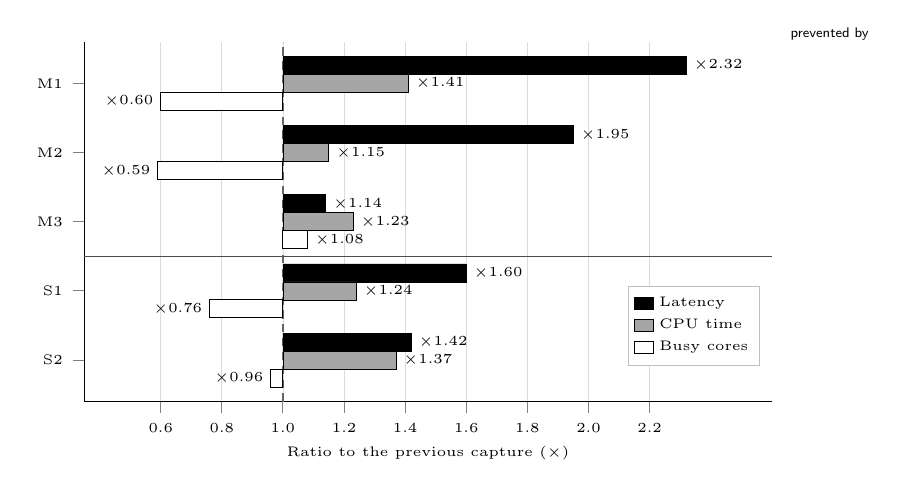
\begin{tikzpicture}
    \newcommand{\rqtwovalr}[4]{%
      \node[font=\tiny,inner sep=0pt,anchor=west,yshift=#1,xshift=2.5pt]
        at (axis cs:#2,#3) {$\times$#4};}
    \newcommand{\rqtwovall}[4]{%
      \node[font=\tiny,inner sep=0pt,anchor=east,yshift=#1,xshift=-2.5pt]
        at (axis cs:#2,#3) {$\times$#4};}
    \begin{axis}[
      xbar,
      bar width=6.5pt,
      y=25pt,
      scale only axis=true,
      width=0.720\columnwidth,
      ymin=0.4, ymax=5.6,
      ytick={1,2,3,4,5},
      yticklabels={S2,S1,M3,M2,M1},
      xmin=-0.65, xmax=1.60,
      xtick={-0.4,-0.2,0,0.2,0.4,0.6,0.8,1.0,1.2},
      xticklabels={0.6,0.8,1.0,1.2,1.4,1.6,1.8,2.0,2.2},
      xlabel={Ratio to the previous capture ($\times$)},
      axis x line*=bottom,
      axis y line*=left,
      tick align=outside,
      xmajorgrids,
      grid style={black!14,line width=0.3pt},
      axis line style={line width=0.35pt},
      tick style={line width=0.35pt},
      tick label style={font=\tiny},
      label style={font=\tiny},
      xlabel style={yshift=2pt},
      legend style={
        font=\tiny,
        draw=black!25,
        fill=white,
        line width=0.2pt,
        inner sep=2pt,
        row sep=-1pt,
        at={(axis cs:1.56,1.5)},
        anchor=east,
        legend columns=1,
        /tikz/every even column/.append style={column sep=3pt},
      },
      legend cell align=left,
      legend image code/.code={%
        \draw[#1] (0cm,-0.075cm) rectangle (0.24cm,0.075cm);},
      clip=false,
    ]

    \draw[black!60,densely dashed,line width=0.5pt]
      (axis cs:0,0.4) -- (axis cs:0,5.6);
    \draw[black!70,line width=0.6pt]
      (axis cs:-0.65,2.5) -- (axis cs:1.60,2.5);

    \addplot[draw=black,fill=black,line width=0.3pt,bar shift=6.5pt]
      coordinates {(1.32,5) (0.95,4) (0.14,3)
                   (0.60,2) (0.42,1)};
    \addlegendentry{Latency}

    \addplot[draw=black,fill=black!35,line width=0.3pt,bar shift=0pt]
      coordinates {(0.41,5) (0.15,4) (0.23,3)
                   (0.24,2) (0.37,1)};
    \addlegendentry{CPU time}

    \addplot[draw=black,fill=white,line width=0.35pt,bar shift=-6.5pt]
      coordinates {(-0.40,5) (-0.41,4) (0.08,3)
                   (-0.24,2) (-0.04,1)};
    \addlegendentry{Busy cores}

    \rqtwovalr{6.5pt}{1.32}{5}{2.32}
    \rqtwovalr{6.5pt}{0.95}{4}{1.95}
    \rqtwovalr{6.5pt}{0.14}{3}{1.14}
    \rqtwovalr{6.5pt}{0.60}{2}{1.60}
    \rqtwovalr{6.5pt}{0.42}{1}{1.42}

    \rqtwovalr{0pt}{0.41}{5}{1.41}
    \rqtwovalr{0pt}{0.15}{4}{1.15}
    \rqtwovalr{0pt}{0.23}{3}{1.23}
    \rqtwovalr{0pt}{0.24}{2}{1.24}
    \rqtwovalr{0pt}{0.37}{1}{1.37}

    \rqtwovall{-6.5pt}{-0.40}{5}{0.60}
    \rqtwovall{-6.5pt}{-0.41}{4}{0.59}
    \rqtwovalr{-6.5pt}{0.08}{3}{1.08}
    \rqtwovall{-6.5pt}{-0.24}{2}{0.76}
    \rqtwovall{-6.5pt}{-0.04}{1}{0.96}

    \node[font=\tiny,inner sep=0pt,anchor=south west]
      at (axis cs:1.66,5.62) {\textsf{prevented by}};
    \rqtwosg{5}{watchdog}
    \rqtwosg{4}{watchdog}
    \rqtwosgtwo{3}{later single-frame}{skip}
    \rqtwosgtwo{2}{earlier multi-frame}{skip}
    \rqtwosgtwo{1}{earlier multi-frame}{skip}

    \end{axis}
  \end{tikzpicture}
   \caption{Reason about each unsafe admit of Table~\ref{tab:rq3_admission_audit}}
  \label{fig:rq3_unsafe_spike_anatomy}
\end{figure}


\subsection{RQ4: Pacing under Queue Pressure}
\label{sec:rq4}

% Notes: docs/exhibits.md#tab_rq4_pacing_sizing
\begin{table}[t]
  \caption{RQ4 Pacing-Delay Sizing under Backlog Pressure.}
  \label{tab:rq4_pacing_sizing}
  \centering
  \scriptsize
  \setlength{\tabcolsep}{2.6pt}
  \renewcommand{\arraystretch}{1.08}
  \resizebox{\columnwidth}{!}{%
  \begin{tabular}{l|r|r|r|r|r|r}
    \toprule
    \multicolumn{1}{c|}{\multirow[c]{3}{*}{\makecell[c]{\textbf{Condition}}}}
    & \multicolumn{4}{c|}{\textbf{Paced by reservation-to-TTL band}}
    & \multicolumn{1}{c|}{\multirow[c]{3}{*}{\makecell[c]{\textbf{$d/B$}\\\textbf{P50}}}}
    & \multicolumn{1}{c}{\multirow[c]{3}{*}{\makecell[c]{\textbf{Overlap}\\\textbf{backlog}}}} \\
    & \multicolumn{4}{c|}{\textbf{\% (counts)}} & & \\
    \cmidrule(lr){2-5}
    & \multicolumn{1}{c|}{{\boldmath\raisebox{0.15ex}{$\scriptstyle <$}}\textbf{60\%}}
    & \multicolumn{1}{c|}{\textbf{60--80\%}}
    & \multicolumn{1}{c|}{\textbf{80--100\%}}
    & \multicolumn{1}{c|}{{\boldmath\raisebox{0.15ex}{$\scriptstyle \geq$}}\textbf{100\%}}
    & & \\
    \midrule
    12MP norm. & \makecell[cr]{\textbf{1.3\%}\\{\tiny $(7/551)$}} & \makecell[cr]{18.1\%\\{\tiny $(62/343)$}} & \makecell[cr]{57.0\%\\{\tiny $(151/265)$}} & \makecell[cr]{\textbf{95.3\%}\\{\tiny $(243/255)$}} & \makecell[cr]{12.5\%} & \makecell[cr]{99.1\%} \\
    \cmidrule(lr){1-7}
    24MP mem. & \makecell[cr]{\textbf{9.6\%}\\{\tiny $(55/572)$}} & \makecell[cr]{32.8\%\\{\tiny $(144/439)$}} & \makecell[cr]{62.2\%\\{\tiny $(240/386)$}} & \makecell[cr]{\textbf{89.1\%}\\{\tiny $(139/156)$}} & \makecell[cr]{13.2\%} & \makecell[cr]{96.9\%} \\
    \bottomrule
  \end{tabular}%
  }
\end{table}

Table~\ref{tab:rq4_pacing_sizing} evaluates 3{,}050 pacing decisions from 116 \emph{Full} runs in the 12MP normal condition, pooled over both devices.
Panel~(a) groups decisions by the backlog \(B_i\) measured from the completed trace, as a fraction of the Capture Timeout budget.
Because backlog is also the pacing rule's dominant term, these bands describe its response rather than test it independently.
Panel~(b) reports pacing coverage for captures whose slack, the deadline margin left at draft sequence completion, fell below 20\%, 10\%, and 5\% of the budget.
For paced decisions, \(d_i/B_i\) is the pacing delay relative to the backlog.

\smallskip\noindent\textbf{Queue response.}
Pacing activation increased sharply with backlog, from 0\% below 10\% of the budget to 8.2\%, 45.0\%, and 83.4\% in successively higher bands.
Among paced decisions, median \(d_i/B_i\) decreased from 29.1\% in the lightest active band to 13.0\% and 8.3\% as backlog increased.
Pacing therefore scaled with queue pressure mainly through more frequent activation rather than larger relative delays.

\smallskip\noindent\textbf{Selective pacing under pressure.}
High backlog alone was not sufficient to trigger pacing.
In the \(\geq 50\%\) backlog group, 574 of 688 decisions were paced, leaving 114 unpaced.
Of these 114, 58 were observed predominantly at lower overheat levels and were projected to fit within the deadline without pacing.
For the other 56, an admission skip had reduced the projected remaining draft work enough to fit within the deadline.

Pacing was more frequent among captures that finished closer to the deadline.
Among captures with slack below 20\%, 10\%, and 5\% of the budget, pacing engaged on 85.4\%, 92.3\%, and 95.7\%, respectively.
The six unpaced captures in the tightest group were backlog-underestimation misses at the pacing decision, but later admission skips kept each capture within budget.
Despite this high near-deadline coverage, median pacing delay was only about 10\% of the queued backlog.
\subsection{Case Study}
\label{sec:casestudy}

% Case study: pre-registered session-selection protocol and the position of the
% selected sessions within their own condition.
%
% Implementation source: private ML repository commit
% 99aae0af8c3fa1ceb784083446e83c40d0fb917f (2026-08-04).
% Workbooks (implementation-repository relative):
%   data/0803_FULL/SM-S948U_metrics_12MP_normal_0803.xlsx
%   data/0803_FULL/SM-S948U_metrics_24MP_memory_0803.xlsx
%
% Both panels are produced by scripts/export_casestudy.py, which fails unless
% the criteria leave exactly one session per condition.  Per-shot traces are in
% data/casestudy/*.csv; the peer statistics are in
% data/casestudy/*_peer_comparison.csv.

\begin{table}[t]
  \centering
  \setlength{\abovecaptionskip}{2pt}%
  \setlength{\belowcaptionskip}{3pt}%
  \caption{Case-study session selection. The criteria are applied before
  inspecting outcomes and leave exactly one session in each condition; the
  12MP session is the one shown in Fig.~\ref{fig:casestudy_12mp}.}
  \label{tab:casestudy_selection}

  {\scriptsize
  \renewcommand{\arraystretch}{1.06}%
  \setlength{\tabcolsep}{3.5pt}%
  \begin{tabular}{|l||r|r|}
    \hline\hline
    \multicolumn{1}{|c||}{\multirow{2}{*}{\textbf{Selection step}}} &
    \multicolumn{2}{c|}{\textbf{Sessions remaining}} \\
    \cline{2-3}
    & \multicolumn{1}{c|}{\makecell[c]{\textbf{12MP}\\\textbf{normal}}}
    & \multicolumn{1}{c|}{\makecell[c]{\textbf{24MP mode +}\\\textbf{memory}}} \\
    \hline\hline
    Recorded sessions & 44 & 44 \\
    \hline
    C1~~30 captures, no Capture Timeout & 43 & 38 \\
    \hline
    C2~~pacing precedes the first demotion & 28 & 20 \\
    \hline
    C3~~\(M\) and \(S\) demoted at distinct captures & 4 & 4 \\
    \hline
    C4~~pacing relaxes to \(0\) for \(\ge 2\) captures & 1 & 2 \\
    \hline
    C5~~pacing reactivates before the \(S\) demotion & 1 & 2 \\
    \hline
    C6~~no Lv5 MP12 resolution fallback\rlap{$^{\dagger}$} & 1 & 1 \\
    \hline\hline
    \textbf{Selected session} &
    \makecell[r]{Run 30\\(Lv4)} & \makecell[r]{Run 34\\(Lv3)} \\
    \hline\hline
    \multicolumn{3}{c}{} \\[-7pt]
    \hline\hline
    \multicolumn{1}{|c||}{\multirow{2}{*}{\textbf{Outcome vs.\ same-condition sessions}}} &
    \multicolumn{2}{c|}{\textbf{Selected / median [min--max]}} \\
    \cline{2-3}
    & \multicolumn{1}{c|}{\(n_p=10\)} & \multicolumn{1}{c|}{\(n_p=6\)} \\
    \hline\hline
    Cumulative applied delay (s) &
      \makecell[r]{5.21 / 4.41\\{}[2.93--8.38]} &
      \makecell[r]{4.39 / 4.23\\{}[2.69--6.62]} \\
    \hline
    Paced transitions (\%) &
      \makecell[r]{55.2 / 43.1\\{}[20.7--75.9]} &
      \makecell[r]{31.0 / 39.7\\{}[13.8--58.6]} \\
    \hline
    Deadline margin \(P_5\) (ms) &
      \makecell[r]{366 / 429\\{}[209--718]} &
      \makecell[r]{302 / 332\\{}[157--769]} \\
    \hline
    Burst span (s) &
      \makecell[r]{21.7 / 20.8\\{}[16.9--22.5]} &
      \makecell[r]{22.8 / 22.7\\{}[19.7--27.3]} \\
    \hline
    \(M\)~executed (\%) &
      \makecell[r]{26.7 / 38.3\\{}[23.3--100]} &
      \makecell[r]{16.7 / 33.3\\{}[10.0--73.3]} \\
    \hline
    \(S\)~executed (\%) &
      \makecell[r]{73.3 / 100\\{}[73.3--100]} &
      \makecell[r]{53.3 / 100\\{}[53.3--100]} \\
    \hline\hline
  \end{tabular}}

  \par\vspace{2pt}
  \begin{minipage}{0.98\columnwidth}
  {\scriptsize \(^{\dagger}\)Binding only in 24MP mode, where Lv5--6 sessions
  use the production MP12 fallback; the 12MP condition has no such fallback.
  Peer sets hold the condition, the starting overheat level, and the capture
  size bucket of the selected session fixed, keep only complete timeout-free
  sessions, and include the selected session itself. In both conditions the
  selected session pays more cumulative pacing delay, holds a smaller
  fifth-percentile deadline margin, spans a longer burst, and completes less
  optional work than its peer median, and it sits at the bottom of its peer set
  for Filter completion; the only metric on the favourable side of the median
  is the paced-transition share of the 24MP session. The sessions were selected
  for mechanism coverage, not for performance. The 24MP-mode column is retained
  to show that the same criteria, applied to a different capture condition,
  again converge on a single session that reproduces the same coordination
  sequence (pacing at capture~4, \(M\) demoted at~6, pacing relaxed over
  captures~6--8, reactivated at~9, \(S\) demoted at~17, no Capture Timeout).
  \par}
  \end{minipage}
\end{table}

% Notes: docs/exhibits.md#fig_casestudy_12mp
\begin{figure}[t]
  \centering
  \setlength{\abovecaptionskip}{2pt}%
  \setlength{\belowcaptionskip}{2pt}%
  \providecommand{\caseStudyDataDir}{data/case_study}
  \providecommand{\csTimeoutRange}[2]{%
    \fill[cs tmo range] ({axis cs:#1,0}|-{rel axis cs:0,0})
      rectangle ({axis cs:#2,0}|-{rel axis cs:0,1});}
  \tikzset{
    cs tmo range/.style={red!70!black,opacity=0.10},
  }
  \pgfplotsset{
    cs executed/.style={
      only marks,mark=square*,mark size=1.35pt,
      draw=black,fill=black!72,line width=0.4pt,
    },
    cs skipped/.style={
      only marks,mark=square,mark size=1.35pt,
      draw=black!45,line width=0.4pt,
    },
    cs delay/.style={
      ybar,bar width=2.1pt,
      draw=blue!55!black,fill=blue!55!black,fill opacity=0.55,line width=0.35pt,
    },
    cs backlog/.style={
      line width=0.7pt,draw=blue!55!black,
      mark=*,mark size=0.9pt,
      mark options={solid,draw=none,fill=blue!55!black},
    },
    cs slack/.style={
      line width=0.7pt,draw=black!80,
      mark=*,mark size=0.9pt,
      mark options={solid,draw=none,fill=black!80},
    },
    cs floor/.style={red!70!black,line width=0.6pt,densely dashed},
    cs step/.style={
      const plot,no marks,line width=0.65pt,draw=black!80,
    },
  }

  \begin{tikzpicture}
    \begin{groupplot}[
      group style={
        group size=1 by 4,
        vertical sep=3.5pt,
        xticklabels at=edge bottom,
      },
      scale only axis=true,
      width=0.78\columnwidth,
      xmin=0.5,xmax=30.5,
      xtick={5,10,15,20,25,30},
      tick label style={font=\scriptsize},
      label style={font=\scriptsize},
      grid=major,
      major grid style={gray!16,line width=0.2pt},
      axis line style={line width=0.4pt},
      tick style={line width=0.4pt},
      tick align=outside,
      tick pos=left,
      ylabel style={
        at={(axis description cs:-0.15,0.5)},
        anchor=south,
        align=center,
      },
    ]

      \nextgroupplot[
        height=0.115\columnwidth,
        ymin=0.4,ymax=2.6,
        ytick={1,2},
        yticklabels={{\(S\)},{\(M\)}},
        yticklabel style={font=\tiny},
        grid=none,
        clip=false,
      ]
      \csTimeoutRange{8}{12}
      \addplot[cs executed] table[x=shot,y=lane,col sep=comma]
        {\caseStudyDataDir/12mp_normal_bokeh_exec.csv};
      \addplot[cs skipped] table[x=shot,y=lane,col sep=comma]
        {\caseStudyDataDir/12mp_normal_bokeh_skip.csv};
      \addplot[cs executed] table[x=shot,y=lane,col sep=comma]
        {\caseStudyDataDir/12mp_normal_filter_exec.csv};
      \addplot[cs skipped] table[x=shot,y=lane,col sep=comma]
        {\caseStudyDataDir/12mp_normal_filter_skip.csv};
      \node[anchor=south,font=\tiny,align=center,
            text=red!70!black,inner sep=1pt]
        at ([yshift=1pt]axis cs:10,2.6)
        {baseline\\first-timeout window};

      \nextgroupplot[
        height=0.135\columnwidth,
        ylabel={Draft Sequence\\queue depth},
        ymin=0,ymax=6.8,
        ytick={0,3,6},
      ]
      \csTimeoutRange{8}{12}
      \addplot[cs step] table[x=shot,y=queue_depth,col sep=comma]
        {\caseStudyDataDir/12mp_normal_backlog.csv};

      \nextgroupplot[
        height=0.22\columnwidth,
        ylabel={Applied delay\\(ms)},
        ymin=0,ymax=1100,
        ytick={0,500,1000},
      ]
      \csTimeoutRange{8}{12}
      \addplot[cs delay] table[x=shot,y=delay_ms,col sep=comma]
        {\caseStudyDataDir/12mp_normal_delay.csv};

      \nextgroupplot[
        height=0.40\columnwidth,
        xlabel={Capture index within the 30-shot run},
        ylabel={\% of\\Capture Timeout},
        ymin=-11,ymax=80,
        ytick={0,20,40,60},
        yticklabels={0\%,20\%,40\%,60\%},
        legend style={
          at={(0.995,0.995)},anchor=north east,
          font=\tiny,draw=none,
          fill=white,fill opacity=0.75,text opacity=1,
          inner xsep=2pt,inner ysep=1pt,
          legend columns=2,
          /tikz/every even column/.append style={column sep=4pt},
        },
        legend cell align=left,
      ]
      \csTimeoutRange{8}{12}
      \addplot[cs floor,forget plot] coordinates {(0.5,0) (30.5,0)};
      \node[anchor=north east,font=\tiny,text=red!70!black,inner sep=1.5pt]
        at ([xshift=-1pt,yshift=-1pt]axis cs:30.5,0)
        {Capture Timeout (Slack \(=0\%\))};
      \addplot[cs backlog] table[x=shot,y expr={\thisrow{backlog_ms}/70},col sep=comma]
        {\caseStudyDataDir/12mp_normal_backlog.csv};
      \addlegendentry{Backlog}
      \addplot[cs slack] table[x=shot,y expr={\thisrow{margin_ms}/70},col sep=comma]
        {\caseStudyDataDir/12mp_normal_margin.csv};
      \addlegendentry{Slack}
      \node[anchor=east,font=\tiny,inner sep=1.5pt] at (axis cs:7.7,2.5)
        {2.1\%};
      \node[anchor=west,font=\tiny,inner sep=1.5pt] at (axis cs:24.4,5.1)
        {5.1\%};
    \end{groupplot}

    \matrix[
      matrix of nodes,
      nodes={font=\tiny,anchor=west,inner ysep=0.4pt},
      column sep=2pt,row sep=0.6pt,anchor=south east,
    ] at ([xshift=5pt,yshift=-2pt]group c1r1.north east) {
      \node[rectangle,draw=black,fill=black!72,line width=0.4pt,
            minimum size=2.7pt,inner sep=0pt] at (0.12,0) {}; & stage executed \\
      \node[rectangle,draw=black!45,line width=0.4pt,
            minimum size=2.7pt,inner sep=0pt] at (0.12,0) {}; & stage skipped by admission \\
    };
  \end{tikzpicture}
  \caption{Case study: stage execution, applied delay, backlog, and slack.}
  \label{fig:casestudy_12mp}
\end{figure}


Table~\ref{tab:casestudy_selection} summarizes the case-study setting and compares the run with its peers.
We selected this run to examine pacing activation, relaxation, and reactivation alongside admission skips.
Its stage-execution counts and slack \(P_5\) are below the peer medians, while both pacing costs are higher.
Figure~\ref{fig:casestudy_12mp} traces these interactions over 30 captures.

\smallskip\noindent\textbf{Control interaction.}
The trace shows a clear division of labor between the two controls.
Admission persistently reduced draft work, while pacing selectively delayed subsequent captures under queue pressure.

Pacing began at capture 5, before slack became critical.
Backlog continued to rise more slowly, but slack still narrowed to 2.1\% of the timeout budget by capture 8.
Admission then began skipping an optional stage at capture 9.
Backlog declined from capture 10, and slack recovered to 27.3\% by capture 15.
Pacing was inactive over captures 13--20 while the stage remained skipped.
Thus, the controller reduced persistent draft work without continuing to add capture delay.

When backlog grew again, pacing resumed at capture 21 and admission began skipping another optional stage at capture 23.
Backlog then declined from its 63.8\% peak, and slack reached 45.6\% by capture 30.
The repeated pattern shows complementary control at two time scales: admission provides persistent workload reduction, while pacing provides reversible timing control as queue pressure changes.
% \subsection{Threats to Validity}
\label{sec:threats}

\smallskip\noindent\textbf{Evaluation scope.}
We evaluated the controller on two devices in Portrait mode with a fixed scene, a 30-capture horizon, and an ADB shutter loop.
Because the controller estimates durations from runtime observations rather than device- or condition-specific timing tables, its behavior depends less on these specific configurations.
The ADB loop also issues requests faster than ordinary shooting, so our runs stress queueing more than typical use.
Broader validation across devices, capture modes, scenes, and additional image-processing stages remains future work.

\smallskip\noindent\textbf{Cold start.}
Both components rely on observed draft sequence durations, so the controller has no prior timing evidence before the first sequence completes.
If that sequence runs unusually long while parallel captures continue to arrive, neither component yet has completed-duration observations with which to estimate the growing processing demand.
We implemented warm-up data support, but left it disabled because no cold-start timeout was observed and maintaining the dataset would add storage and maintenance cost.


\section{Related Work}
\label{sec:related_work}

\smallskip\noindent\textbf{Workload control.}
Our admission controller builds on work that adapts per-input computation at run time under latency, resource, or thermal constraints~\cite{liu-imprecise-computation,shih-imprecise-siam,zilberstein-anytime,loop-perforation-fse,apnet-rtss,branchynet-icpr,msdnet-iclr,mcdnn-mobisys,nestdnn-mobicom,reducto-sigcomm}.
ApproxDet and Chanakya select execution configurations according to input content, resource contention, and latency--accuracy objectives~\cite{approxdet-sensys,chanakya-neurips}.
Recent mobile and embedded systems similarly adapt execution under device constraints: Agile3D selects 3D-detection branches under changing scenes and GPU contention~\cite{agile3d-mobisys}, ARIA coordinates vision inference across heterogeneous mobile processors~\cite{aria-mobisys}, and Phoenix adjusts processor placement and DNN exit depth under thermal throttling~\cite{phoenix-tecs}.
Timecard is closer to our admission logic, tracking each request's elapsed end-to-end budget and adapting its remaining processing to the time left~\cite{timecard-sosp}.
Our admission controller uses a similar budget abstraction, but applies it at stage boundaries, admitting an optional stage only when the remaining draft sequence is still feasible within the capture deadline.
Across this line of work, the control target is the computation performed for the current input.
In our capture pipeline, however, parallel capture can introduce the next capture before the shared draft sequence worker becomes idle.
Reducing current-capture work alone is therefore insufficient.
The pipeline must also control when the next capture is released.

\smallskip\noindent\textbf{Arrival control.}
Our pacing mechanism is related to systems that control request admission or release timing to limit queueing delay~\cite{cruz-network-calculus}.
Networking limits queue growth through active queue management and pacing~\cite{red-floyd-jacobson,codel-cacm,rfc8289,rfc8033,rfc8290,bufferbloat-cacm,tcp-pacing-infocom,bbr-queue}, while server systems admit, reject, or shed requests according to load or deadline signals~\cite{seda-sosp,dagor-socc,breakwater-osdi,aurora-load-shedding,deadline-aware-d3}.
Real-time schedulers similarly regulate job releases by stretching task periods or skipping job instances~\cite{buttazzo-elastic-task,koren-skip-over}.
Preemptive systems can instead interrupt running work to serve short or urgent requests~\cite{shinjuku-nsdi}.
Across these systems, the controller can alter job admission, release, or execution.
In our camera system, a user's shutter press cannot be rejected, and a running stage cannot be preempted.
Our pacing therefore delays next-capture release.
It limits queue growth without reducing work admitted for the current capture.

\smallskip\noindent\textbf{Coordinating workload and arrivals.}
Prior systems have also combined the two control dimensions discussed above.
Feedback-control systems regulate incoming load through request admission while adjusting the service level of admitted requests from deadline-miss or response-time feedback~\cite{lu-feedback-control-edf,lu-feedback-control-scheduling,welsh-overload-control}.
QoS negotiation similarly reduces service quality to accept requests that might otherwise be rejected~\cite{abdelzaher-qos-negotiation}.
These systems control both whether incoming work is accepted and how much service it receives, with rejection remaining one of their control actions.
Content adaptation and brownout instead reduce per-request work without controlling when requests arrive~\cite{abdelzaher-content-adaptation,klein-brownout}.
Neither pattern directly matches our capture pipeline: once issued, a user-triggered capture must be served rather than rejected, and reducing current-capture work alone is insufficient under parallel capture.
Our controller therefore couples the two controls across consecutive captures: admission decides which optional stages the current capture executes, while pacing delays the release of the next capture instead of rejecting it.
To our knowledge, this is the first work to combine per-capture remaining-budget admission with next-capture pacing in a production camera system under a hard per-capture deadline.
\section{Conclusion}

\label{sec:conclusion}

% Under parallel capture, lightweight multi-frame composition in the draft sequence creates a cross-capture deadline problem. 
% Work admitted for one capture reduces the budget available to subsequent captures on the serialized, non-preemptible Draft worker.
% This paper presents the Budget-Aware Draft Controller, which coordinates remaining-sequence admission with capture-availability pacing using runtime duration observations.
% Across 28 evaluated cells, every full-controller run completed the 30-capture horizon without an observed Capture Timeout, whereas the unguarded baseline timed out in 26 cells. 
% The controller also retained optional processing above the production thermal cutoff.
% These results support coordinated workload and arrival control as a practical alternative to static feature suppression in deadline-constrained, serialized pipelines.

\bibliographystyle{IEEEtran}
\bibliography{refs}

\end{document}
